\chapter{Physics objects}
\label{sec:objects}

In this section, a list of the physics objects used in the analysis is presented, together with performance and validation plots. 

The objects are selected according to the standard Run2 reccomendations provided by the various POGs for the Summer16 (25ns) MiniAOD-v2 (Moriond reccomendations).

The version of CMSSW used for the analysis is {\tt CMSSW\_8\_0\_25}.

\section{Vertex and Pile-up}
{\color{red} How the vertices and pile-up are reconstructed}

Due to pileup several primary vertices are typically reconstructed in an event.
The primary vertex of the event is defined as the one with the highest sum of transverse momenta $\sum \pt^2$ of clustered physics objects associated to it, which passes the following selections:
\begin{itemize}
  \item number of degrees of freedom $N_{DoF}>4$
  \item vertex position along the beampipe $|z_{vtx}|<24\cm$
  \item vertex distance with respect the beam pipe $d_0<2\cm$
\end{itemize}
where $z_{vtx}$ and $d_0$ are the distance along and perpendicular to the beam line of the vertex with respect the nominal interaction point $(0,0,0)$.

The data sample contains a significant number of additional interactions per bunch crossing, an effect known as pileup (PU). 

The {\tt Summer16} \texttt{v2} MINIAOD Monte Carlo samples are generated simulating the PU conditions, using the 25ns asymptotic PU scenario. 
Nevertheless, the MC PU description does not match exactly the conditions in data, and there is therefore the need to reweight the simulated events in order to improve the agreement with the data. 

The MC samples are reweighted using the standard CMS PU reweighting technique~\cite{bib:pureweight,bib:pureweight2} assuming a total inelastic cross section of $\sigma_{in} = 69\,200 \mu b$.

The comparison between the distributions of primary vertices in data and MC after the PU reweighting is applied is shown in Figure~\ref{fig:npv} for an event selection (called inclusive selection) requiring large amount of \met recoiling against an AK8 fat jet~(Tab.~\ref{tab:sel}).
 
 \begin{figure}[!htb]
  \centering
    %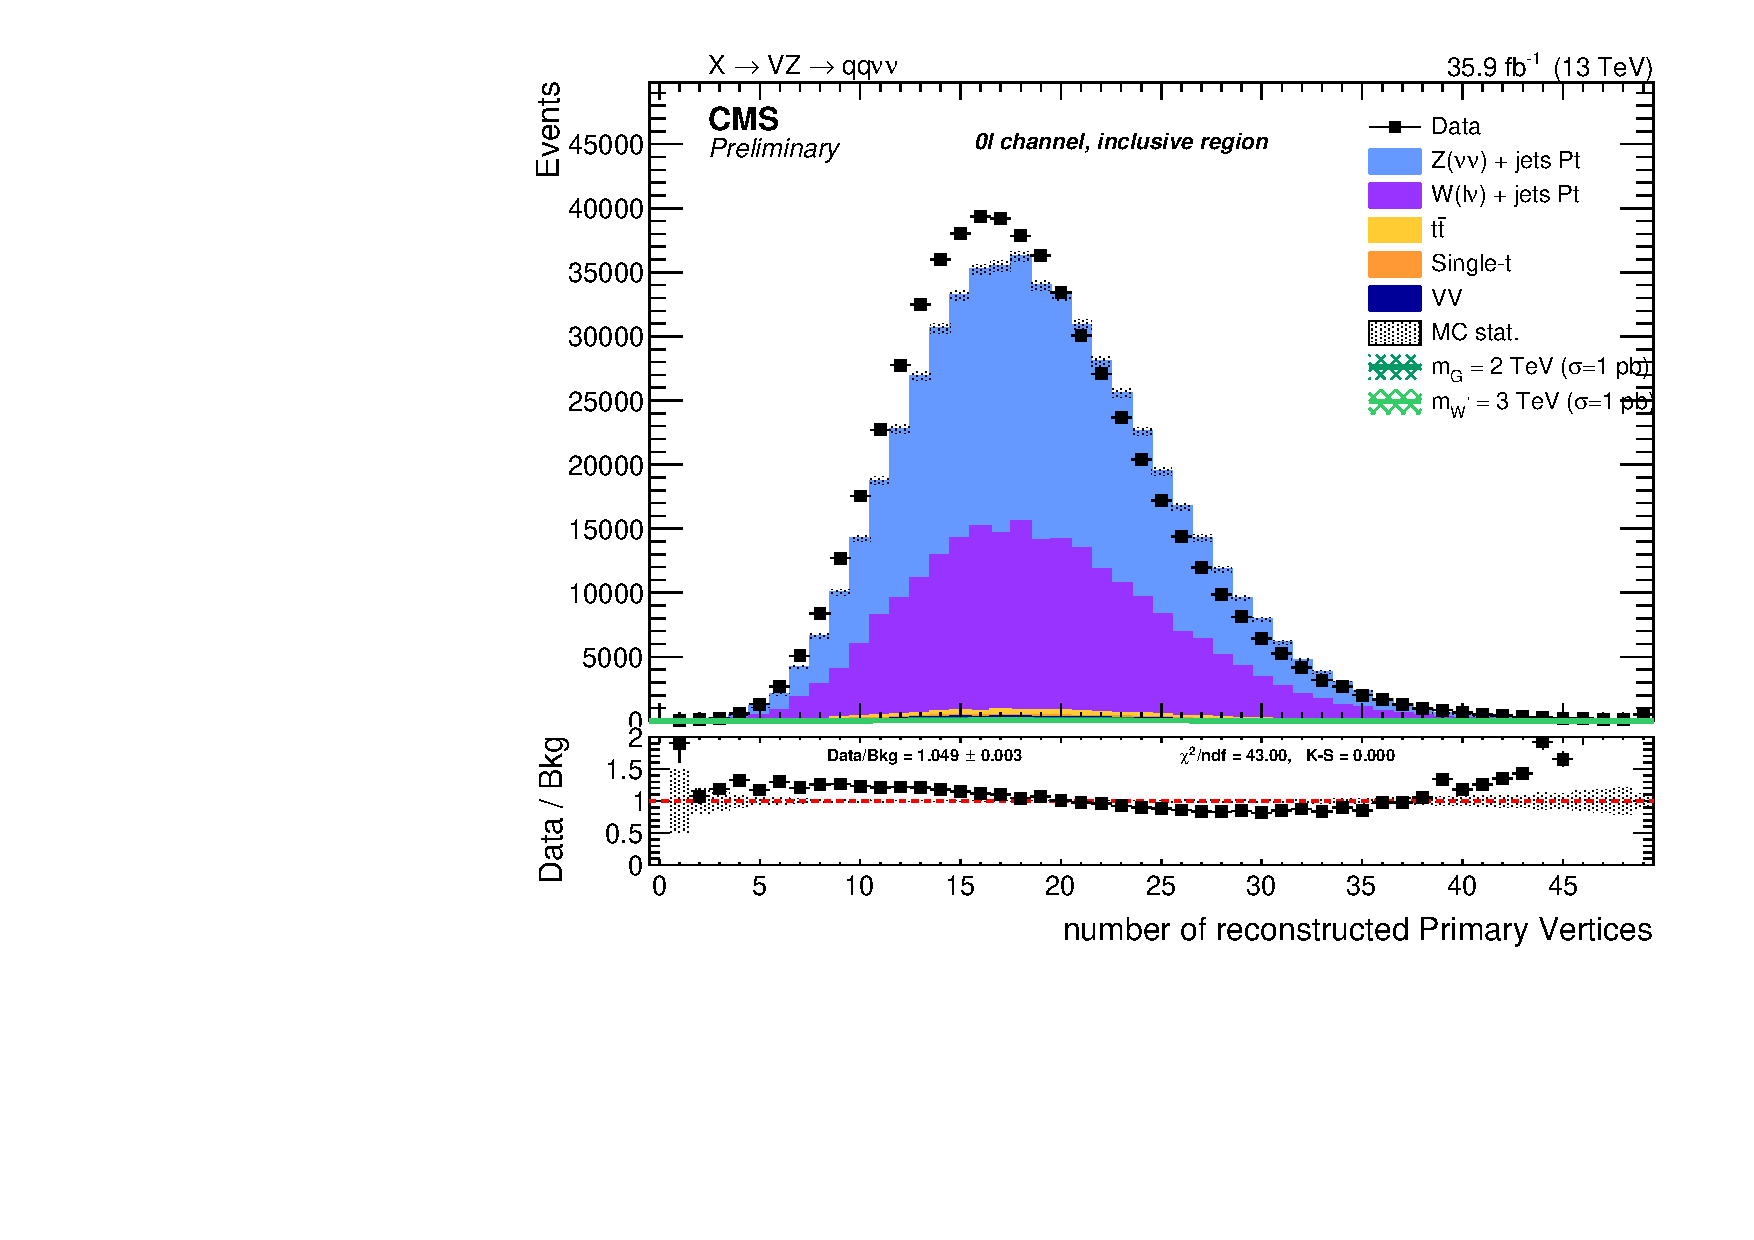
\includegraphics[width=.495\textwidth]{plots/v9_U/XVZnnInc/nPV.pdf}
  \caption{Primary vertices distributions after reweighting with the official recipe and $\sigma_{in}=69\,200 \mu b$.}
  \label{fig:npv}
 \end{figure}


\section{Electrons}\label{ssec:electrons}
{\color{red} How the electrons are reconstructed}

Electrons are reconstructed from energy deposits in the ECAL matched to tracks reconstructed in the silicon tracker. 
The electron trajectories are reconstructed using a dedicated modeling of the electron energy loss and fitted with a Gaussian sum filter.
Electrons used in this analysis are required to pass the Particle Flow criteria, and to fall in the ECAL pseudorapidity fiducial range ($|\eta|<2.5$). 

The electron identification used in this analysis is based on the ``cut-based'' Id defined by the EGamma POG for the \texttt{Summer16} 25ns~\cite{EGammaPOG_ele}, and suggested also for the usage in 80X for the so-called Moriond dataset.
Isolation cuts are already applied within the cut-based Id definitions, therefore no additional Isolation cut is required.
In the isolation definition the effect of PU is considered by taking into account the energy deposits in the calorimeter, estimated through the so-called \emph{$\rho$-area} method, by subtracting the median energy density in the event $\rho$ multiplied by electron effective area.
The isolation value is computed in a $\Delta$R cone of 0.3 centered along the lepton direction.

Since in this analysis we are aiming at a final state without any lepton, every electron identified with \emph{veto} cut-based Id, transverse momentum $\pt > 10$ GeV is vetoed. The detailed set of cuts to define a \emph{veto} cut-based Id electron are reported in the Table~\ref{tab:EGcutBar}.

%The detailed set of cuts are reported in the Table~\ref{tab:EGcutBar}. $\Delta \eta_{in}^{seed}$ and $\Delta \varphi_{in}$ are the difference in $\eta$ and $\varphi$ between the track position as measured in the inner layer, extrapolated to the interaction vertex and then extrapolated to the calorimeter and the $\eta$ of the seed cluster or the $\varphi$ of the supercluster, $H/E$ is the ratio of the hadronic energy of the CaloTowers in a cone of radius 0.15 centred on the electron's position in the calorimeter to the electromagnetic energy of the electron's supercluster, $\sigma_{i\eta i\eta}$ is the spread in eta in units of crystals of the electrons energy in 5x5 block centred on the seed crystal, and $1/E - 1/p$ is the difference of the inverse of the energy and the momentum.
% $E^{2x5}/E^{5x5}$ is fraction of energy in 2x5 crystals around seed to the energy in 5x5 crystals around the seed, 

\begin{table}[htb]
 \centering
    \begin{tabular}{lccc}
     \hline

    Electrons                   &        & \multicolumn{2}{c}{\texttt{Veto}}\\
                                &        & EB      & EE     \\
 \hline
    $\sigma_{i\eta i\eta} $     & $ < $  &0.0115   &0.037  \\
    $\Delta \eta_{in}^{seed}$   & $ < $  &0.00749  &0.00895 \\
    $\Delta \varphi_{in} $      & $ < $  &0.228    &0.213   \\
    $H/E $                      & $ < $  &0.356    &0.211   \\
    relIso (EA)                 & $<$    &0.175    &0.159   \\
    $|1/E - 1/p|$               & $ < $  &0.299    &0.15    \\
    $|d_0|$                     & $ < $  &0.05     &0.10   \\
    $|d_z|$                     & $ < $  &0.10     &0.20   \\
    missing hits                & $\leq$ &2        &3       \\
    conversion veto             &        &  yes    &yes     \\
    
 \hline
\end{tabular}
\caption{ Summer16 cut-based selection for 25ns conditions. EB: barrel cuts ( $|\eta_\text{supercluster}| \leq 1.479$); EE: endcap cuts ( $|\eta_\text{supercluster}| > 1.479$)}
\label{tab:EGcutBar}
\end{table}

Scale factors for electron identification (including isolation) are provided by Egamma POG, derived for 80X (Moriond 17 recommendation), that can be found in~\cite{EGammaPOG_ele_SF}.


%\clearpage

\section{Muons}\label{ssec:muons}

{\color{red} How the muons are reconstructed}

In the standard CMS reconstruction for $pp$ collisions, muon tracks are first reconstructed independently in the inner tracker (tracker track) and in the muon system (standalone-muon track). Based on these objects, two reconstruction approaches are used~\cite{bib:CMS-PAPER-MUO-10-004}: \emph{Global Muon} (outside-in) and \emph{Tracker Muon} (inside-out).
\begin{itemize}
  \item[\emph{Global Muon reconstruction (outside-in)}:] for each standalone-muon track, a matching tracker track is found by comparing parameters of the two tracks propagated onto a common surface, and a global-muon track is fitted combining hits from the tracker track and standalone-muon track, using the Kalman-filter technique~\cite{bib:kalman}. At large transverse momenta, $\pt > 200 \GeV$, the global-muon fit can improve the momentum resolution compared to the tracker-only fit.
  \item[\emph{Tracker Muon reconstruction (inside-out)}:] in this approach, all tracker tracks with $\pt > 0.5 \GeV$ and the total momentum $p > 2.5 \GeV$ are considered as possible muon candidates and are extrapolated to the muon system taking into account the magnetic field, the average expected energy losses, and multiple scattering in the detector material. If at least one muon segment (i.e., a short track stub made of DT or CSC hits) matches the extrapolated track, the corresponding tracker track qualifies as a Tracker Muon.
\end{itemize}

Tracker Muon reconstruction is more efficient than the Global Muon reconstruction at low momenta, $\pt \lesssim 5 \GeV$, because it requires only a single muon segment in the muon system, whereas Global Muon reconstruction is designed to have high efficiency for muons penetrating through more than one muon station and typically requires segments in at least two muon stations. Thanks to the high tracker-track efficiency and a very high efficiency of reconstructing segments in the muon system, about 99\% of muons produced in $pp$ collisions and having sufficiently high momentum are reconstructed either as a Global Muon or a Tracker Muon, and very often as both. Muons reconstructed only as standalone-muon tracks have worse momentum resolution and less favorable collision muon to cosmic-ray muon ratio than the Global and Tracker Muons and are usually not used in physics analyses.

Muons are usually based on the \emph{Particle Flow Muon} selection, considering Global Muon or a Tracker Muon candidates and by applying minimal requirements on the track components in the muon system and taking into account a matching with small energy deposits in the calorimeters. %However, in the boosted $\Z \to \mu\mu$ regimes, muons have similar problems to electrons. The Global muon reconstruction suffers a drop in efficiency as the $\Delta R$ between the muon decreases. This is a consequence of the seeding algorithm, which includes in the seed some segments of the other muon, and after the final muon trajectory builder, a cleaning is applied based on the number of segments and the $\chi^2$ of the muon track. After the cleaning, only one muon track is selected among the group of tracks that share segments, and this effect avoids the reconstruction of the other muon (Figure~\ref{fig:Muon_Multi}).

%The reconstruction of muons very close in $\Delta R$ is also a problem for the PF algorithm, which is based on the hypothesis that the muon is a minimum-ionizing particle. Another high-\pt track close to a reconstructed muon can also fail to pass the PF identification of the nearby muon, further lowering the efficiency at small angles, as shown in Figure~\ref{fig:Muon_Multi}.
%The adopted compromise between efficiency and fake-muons rejection is then to require that \emph{at least} one of the two muons (not necessarily the highest-\pt) fulfills both the PF and the \texttt{HighPt}, while the other has to satisfy a looser selection. This asymmetric selections ensures a high efficiency ($\gtrsim 95\%$) in the whole \pt, $\eta$ %(Figure~\ref{fig:Muon_pt_eta})
%and $\Delta R$ ranges (Figure~\ref{fig:Muon_Multi}). 
%The \texttt{HighPt} Id is a set of cuts specifically designed for high-momentum muons from the Muon POG~\cite{MuonPOG}:

%\begin{itemize}
%   \item to be reconstructed also as Global muon
%   \item at least one muon chamber hit included in the global-muon track fit
%   \item muon segments in at least two muon stations
%   \item the track used to obtain the muon momentum needs to pass $\delta\pt/\pt < 0.3$
%   \item tracker track transverse impact parameter $d_{xy} < \unit{2}{\text{mm}}$ w.r.t. the primary vertex
%   \item longitudinal impact parameter $d_z < \unit{5}{\text{mm}}$ w.r.t. the primary vertex
%   \item number of pixel hits $>0$
%   \item number of tracker layers with hits $> 5$.
%\end{itemize}

%The other muons in the event, if present, should be identified with a tracker-only selection. A tight \texttt{CustomTracker} Id is defined using the same quality cuts on the muon track as the \texttt{HighPt}, but dropping the requirements that force the muon to be Global or PF:

%\begin{itemize}
%    \item to be reconstructed as a standard Tracker muon (was Global muon in HightPt Id)
%    \item at least one muon chamber hit included in the global-muon track fit
%    \item muon segments in at least two muon stations
%    \item the track used to obtain the muon momentum needs to pass $d\pt/\pt < 0.3$.
%    \item TuneP-track transverse impact parameter $d_{xy} < \unit{2}{\text{mm}}$ w.r.t. the primary vertex (was Tracker-track)
%    \item longitudinal impact parameter $d_z < \unit{5}{\text{mm}}$ w.r.t. the primary vertex
%    \item number of pixel hits $>0$
%    \item number of tracker layers with hits $> 5$.
%\end{itemize}

%Having dropped the PF identification requirements, the best estimation of the muon momentum is then extracted via the TuneP algorithm, better suited for high-\pt muons.

For muons reconstructed using the PF algorithm, the standard muon isolation is defined as the ratio of the \pt sum of all charged and neutral particle-flow candidates in the event within a cone with a radius of $\Delta R=0.4$ centered along the lepton direction. Corrections in order to reduce the PU contamination are also applied, using the $\Delta \beta$ method.
Charged candidates falling into the cone that are not compatible with the primary vertex are removed from the sum. Additionally, the neutral contribution from PU is estimated to be half the one coming from charged candidates, and this quantity is also subtracted from the total. Eventually, the scalar sum is divided by the lepton \pt itself. The general formula for the standard \emph{particle-flow} isolation is then:
$$I_{rel} = \left[ \sum \pt^\text{ch \ had} + \max(\sum \pt^\text{neu \ had} + \sum \pt^{\gamma} - 0.5 \cdot \sum \pt^\text{pu \ ch \ had}, \ 0) \right] /\pt^\ell $$
where $\sum \pt^\text{ch \ had}$ is the sum of the transverse momenta of the charged hadrons, $\sum \pt^\text{neu \ had}$ is the sum of transverse energies of the neutral hadrons, $\pt^{\gamma}$ is the sum of the transverse energy of particle flow photons and $\sum \pt^\text{pu \ ch \ had}$ is the sum of transverse momenta of the charged particles in the cone of interest but with particles not originating from the primary vertex (for pileup corrections). %With this definition of the isolation the other electron of the system does not enter the calculation.

%In the case of muons not reconstructed using the PF algorithm, as in the case of the \texttt{CustomTracker} id used to select muons in this analysis, the MuonPOG provides a Tracker-based definition of isolation.
%This isolation is computed as the scalar sum of the \pt of all the track from the leading PV in the event within a cone with a radius of $\Delta R=0.3$ centered along the muon direction, normalized by the muon \pt.

In the VZ event selection, all muons identified with the \texttt{Loose} standard id, \pt over 10 GeV, PF isolation below 0.25, $\eta<|2.4|$ are vetoed.

%In the VZ event selection, at least one muon is required to be identified with the \texttt{HighPt} standard id, while the other is selected if passes wither the \texttt{CustomTracker} requirements or the standard \texttt{HighPt}. The \emph{loose} working point ($<0.1$) of the tracker-based isolation criterion is used to select the leptons. When evaluating the tracker-isolation for each muon, if the other selected muon falls in the $\Delta R < 0.3$ isolation cone, the tracker-based isolation is recomputed after removing the inner tracker track \pt of the other muon.
 
Scale factors for muon identification and isolation are centrally provided as a function of the muon \pt and $\eta$ by the Muon POG~\cite{MuonSF}, and are applied consistently in the analysis.


\section{Taus}\label{sec:tau}
{\color{red} How the taus are reconstructed}
 
The presence of hadronically-decaying taus only act as veto for the events both in the signal and in the control regions to suppress electroweak backgrounds. The selection criteria for taus are $\pt > 18$ GeV and $|\eta| < 2.3$. The Run2 TauPOG recomended identification criteria~\cite{TauPOG} (\texttt{decayModeFinding}, \texttt{byLooseCombinedIsolationDeltaBetaCorr3Hits})  are required and applied in order to identify possible tau candidates.
% % The tau-lepton multiplicity in the inclusive $\Z \to \mu\mu$ is reported in Fig.~\ref{fig:ZmmInc_taupho}.
% 
\section{Photons}
{\color{red} How the photons are reconstructed}

As in the case of tau leptons, a photon veto is applied in the analysis both for the signal and the control regions.
Events are rejected if they contains one (or more) photon with $\pt > 15$ GeV , $|\eta| < 2.5$, passing the \texttt{Loose} cut-based photon ID. The \texttt{Loose} photon Id is applied as in the EGamma POG recommandations for Run2 analyses~\cite{EGammaPOG_pho} (tuned on \texttt{ Spring16} 25 ns samples).
The isolation cuts (using the rho-area method for the mitigation of the pileup) and conversion safe electron veto are applied.
The isolation value is computed in a $\Delta R$ cone of 0.3 and is corrected for pileup by subtracting the event-by-event energy density ($\rho$) times an effective area.
The applied cut-based definition of the \texttt{Loose} photon Id is reported in Table~\ref{tab:PhotonId}.
% % The photon multiplicity in the inclusive $\Z \to \mu\mu$ is reported in Fig.~\ref{fig:ZmmInc_taupho}.
% 
 \begin{table}[htb]
  \centering
     \begin{tabular}{lccc}
      \hline
 
     Photons                                   &       & \multicolumn{2}{c}{\texttt{Loose}}\\
                                               &       & EB      & EE  \\
  \hline
     $H/E $                                    & $ < $ &0.0597   & 0.0481      \\
     $\sigma_{i\eta i\eta} $                   & $ < $ &0.01031  & 0.03013   \\
     PF ch.had.iso.($\rho$-corr)               & $ < $ &1.295    & 1.011   \\
     PF neu.had.iso.($\rho$-corr)              & $ < $ &$10.910+0.0148\pt+0.000017\pt^2$    &$5.931+0.0163\pt+0.000014\pt^2 $   \\
     PF photon iso.($\rho$-corr)               & $ < $ &$3.630+0.0047\pt$                 &$6.641+0.0034\pt $   \\
     conversion veto                           &       & yes     &yes     \\
  \hline
 \end{tabular}
  \caption{Photon cut-based Id for Spring16 25ns conditions. EB: barrel cuts ( $|\eta_\text{supercluster}| \leq 1.479$); EE: endcap cuts ( $|\eta_\text{supercluster}| > 1.479$)}\label{tab:PhotonId}
 \end{table}

Scale factors for photon identification (including isolation) are provided by Egamma POG, derived for 80X (Moriond 17 recommendation), that can be found in~\cite{EGammaPOG_ele_SF}.

\clearpage


\section{Jets}\label{ssec:jets}
{\color{red} How the jets are reconstructed}

Events in the CMS detector are reconstructed using the particle-flow algorithm~\cite{bib:PF1,bib:PF2}, which combines information from all sub-detectors in order to reconstruct stable particles (muons, electrons, photons, neutral and charged hadrons). The charged hadron subtraction algorithm (CHS) removes candidates not associated to the primary vertex in order to remove contributions from pileup~\cite{CMS-PAS-JME-14-001}. The remaining particles are used as input to jet clustering algorithms to reconstruct particle-flow jets. The jets are clustered using the {\sc FastJet} package~\cite{bib:fastjet} with the anti-\kt jet clustering algorithm~\cite{Cacciari:2008gp} with a clustering parameter of $R = 0.8$ (``fat''-jets or AK8 jets) or $R = 0.4$ (``standard''-jets or AK4 jets). In order to avoid double-counting of PF candidates, AK4 jets are considered only if the angular separation from the leading AK8 jet is larger than $\Delta R>0.8$.
Several levels of jet energy corrections are applied to the momentum of the clustered (raw) jets in order to obtain the energy value that is closer to the true energy of the initial parton~\cite{bib:1748-0221-6-11-P11002}:

\begin{itemize}
  \item[\emph{L1 Offset}:] the pileup and electronic noise effects are removed. This correction can be estimated using events collected by a random trigger, without any preconditions except a beam crossing, referred as \emph{zero bias} events. The offset contribution from pileup is estimated by the FastJet method which relies on the definition of a jet area~\cite{bib:fastjet} from which a median energy density ($\rho$, in \GeV/Area) per event can be defined. The correction subtracted to the jet \pt equals to $\rho$ times the jet area. FastJet has the advantage of being able to remove the out-of-time pileup component, but has the disadvantage of subtracting the underlying event contribution as well.
  \item[\emph{L2 Relative ($\eta$)}:] the variation in jet response with $\eta$ is flattened. The unbalance between the jets transverse momentum that is observed on average, is due to the variation of the jet response across the detector versus $\eta$.
  \item[\emph{L3 Absolute (\pt)}:] the calorimetric energy response varies as a function of the jet \pt. The absolute correction removes these variations and makes the response equal to unity. This correction is obtained from simulation using the Monte Carlo truth information.
  \item[\emph{L2L3 Residual}:] differences between data and simulation after L2 and L3 corrections are removed by applying a specific calibration to data events. Residual corrections are extracted from data using the transverse momentum balance in $\gamma$+jets and \Z+jets events~\cite{bib:1748-0221-6-11-P11002}.
\end{itemize}

The latest jet energy corrections are applied to AK4 and AK8 CHS jets, and the tags are {\tt Summer16 23Sep2016V3}.

In this analysis, jets are considered if the corrected \pt is larger than 30 \GeV for AK4 jets and 200\GeV for AK8 jets, and lie in the tracker acceptance ($|\eta|<2.4$). Additionally, AK4 are required to pass \emph{loose} jet identification requirements, AK8 are required to pass \emph{tight} jet identification requirements defined by the JETMET POG for Run2 analyses~\cite{JetMETPOG}, listed in Table~\ref{tab:JetId}. AK8 jets are used to reconstruct the hadronically decaying electroweak boson candidate, whilst AK4 jets are used to suppress the contribution of top and QCD background events.

Figure~\ref{fig:n_AK8}-~\ref{fig:AK8jet_eta} show the data/simulation comparison after the analysis selections~(Tab.~\ref{tab:sel} without Top cleaning and Event cleaning).

\begin{table}[htb]
 \centering
 \begin{tabular}{lll}
\hline
PF Jet ID                       & \emph{loose}   & \emph{tight}   \\
\hline
Neutral Hadron Fraction         & $< 0.99  $     & $< 0.90  $    \\
Neutral EM Fraction             & $< 0.99  $     & $< 0.90  $\\
Number of Constituents          & $> 1     $     & $> 1     $\\
Muon Fraction                   & \--            & \-- \\
\hline
\multicolumn{3}{l}{Additionally, for $|\eta| < 2.4$ } \\
\hline
Charged Hadron Fraction         & $> 0   $& $> 0   $\\
Charged Multiplicity            & $> 0   $& $> 0   $\\
Charged EM Fraction             & $< 0.99$& $< 0.99$\\
\hline
 \end{tabular}
 \caption{ \emph{Loose} and \emph{Tight} jet identification requirements for Run2 (Spring16) 25ns conditions.\label{tab:JetId}}
\end{table}

\begin{figure}[!htb]
  \begin{center}
    %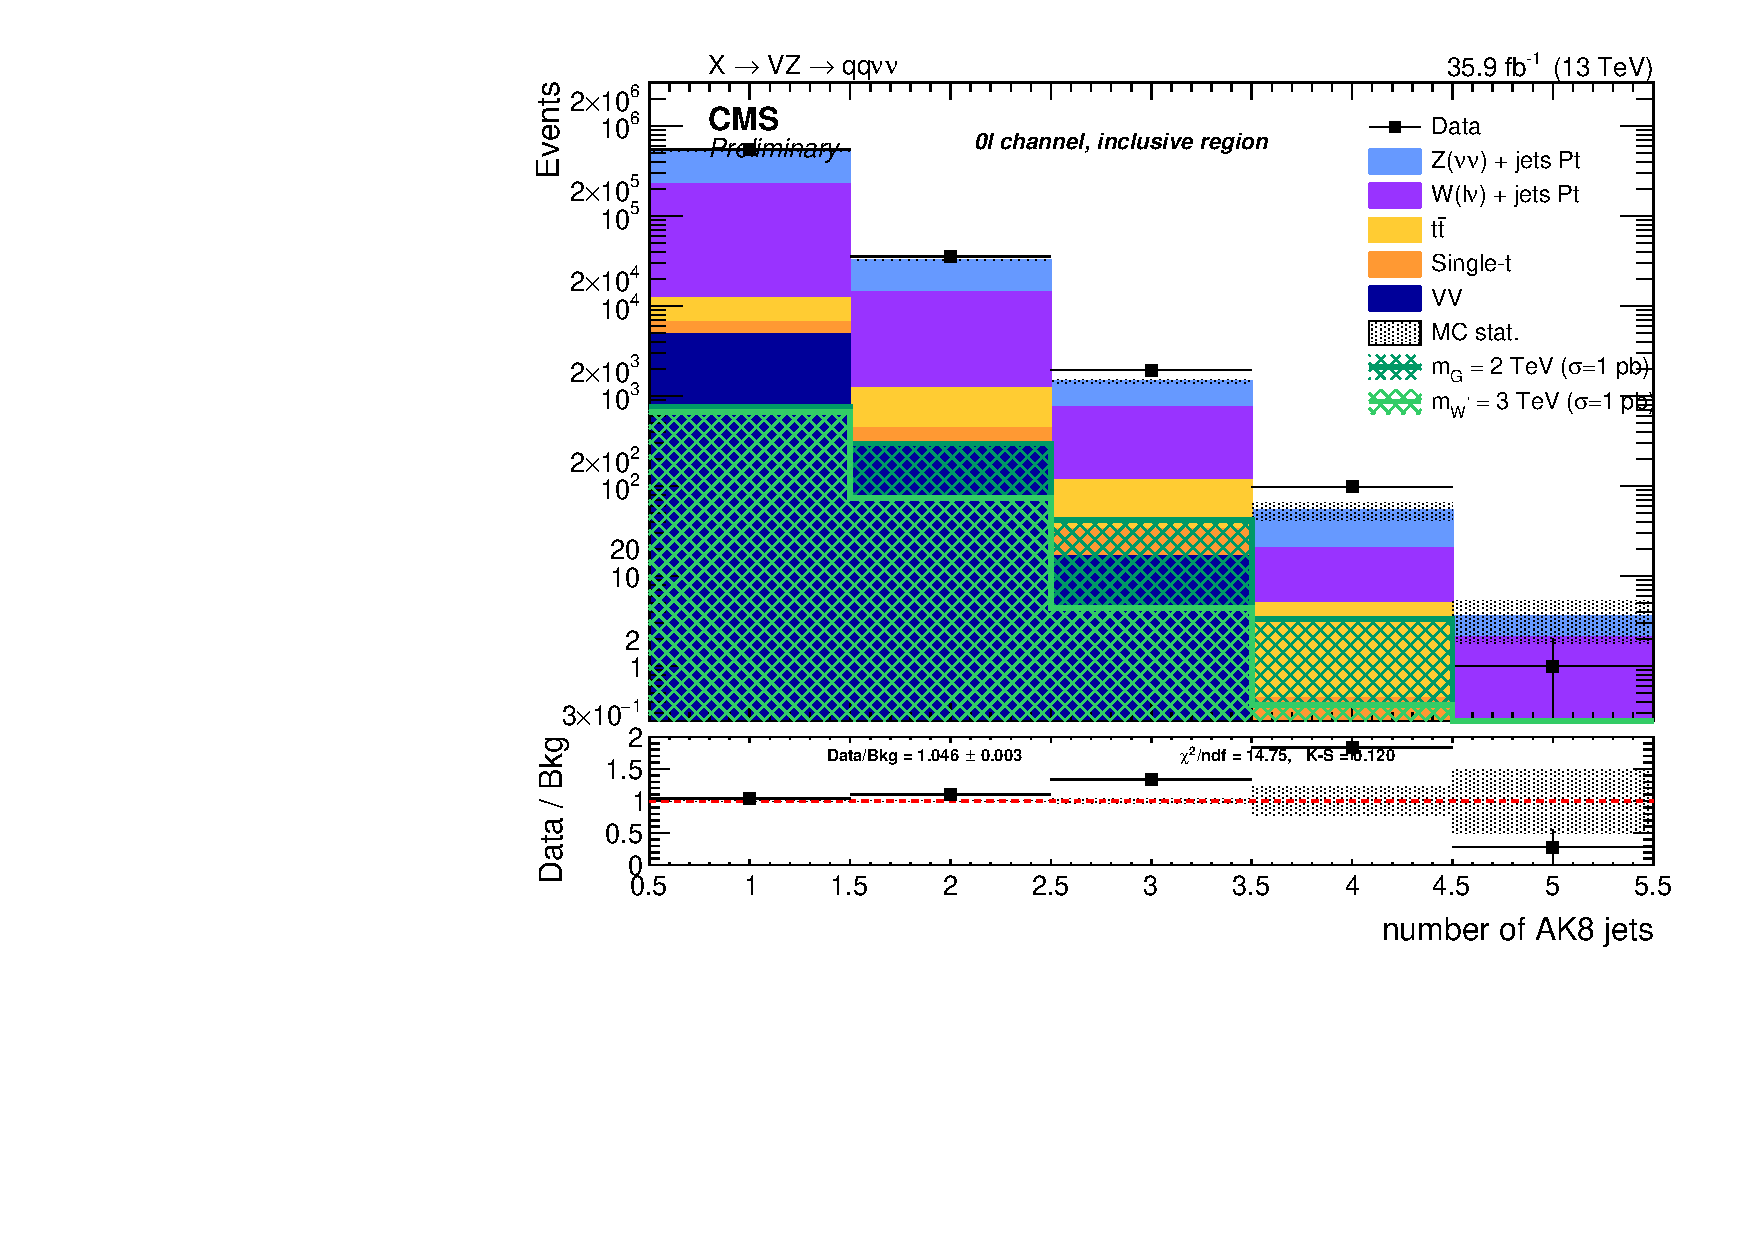
\includegraphics[width=.495\textwidth]{plots/v9_U/XVZnnInc/nFatJets.pdf}
  \end{center}
  \caption{Number of reconstructed AK8 jets after selections.}
  \label{fig:n_AK8}
\end{figure}

\begin{figure}[!htb]
  \begin{center}
    %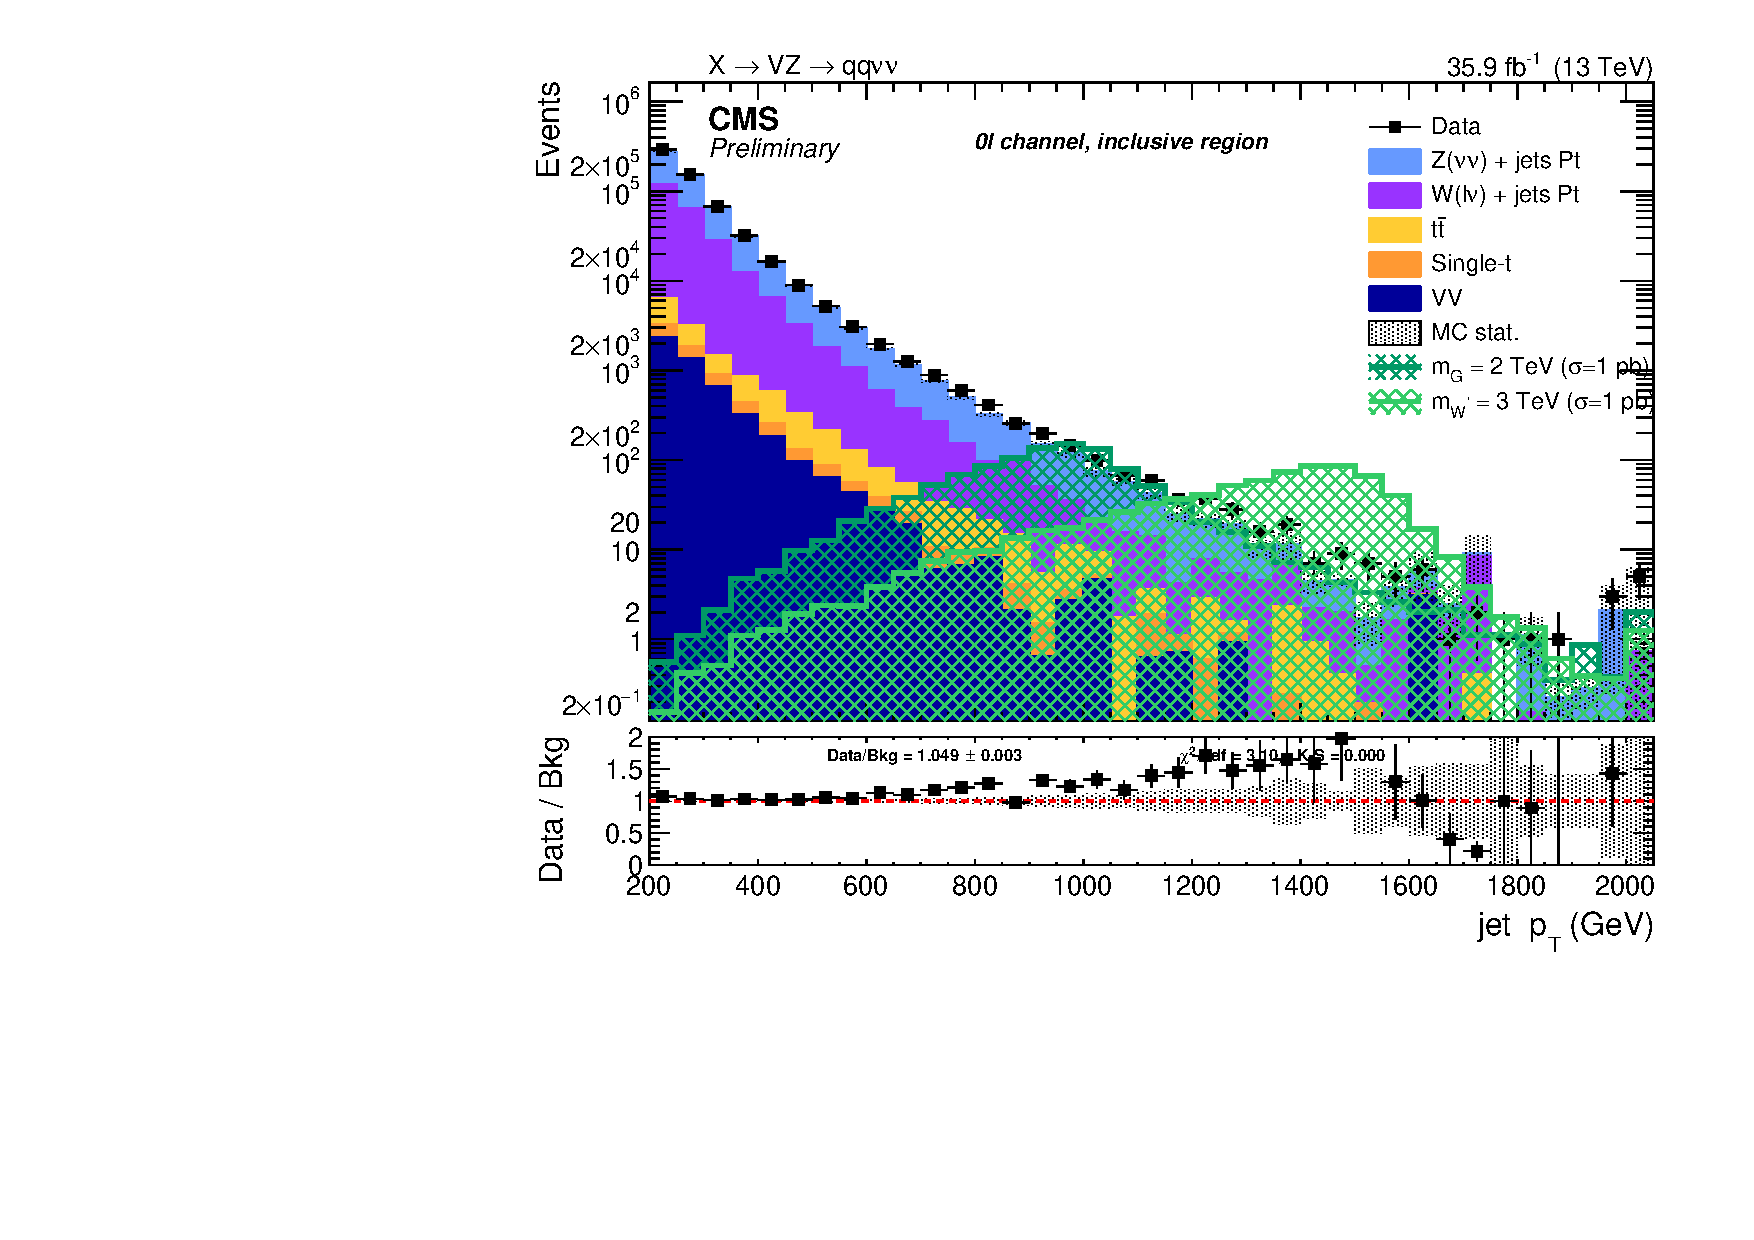
\includegraphics[width=.495\textwidth]{plots/v9_U/XVZnnInc/FatJet1_pt.pdf}
  \end{center}
  \caption{Leading AK8 jet \pt spectra after selections.}
  \label{fig:AK8jet_pt}
\end{figure}

\begin{figure}[!htb]
  \begin{center}
    %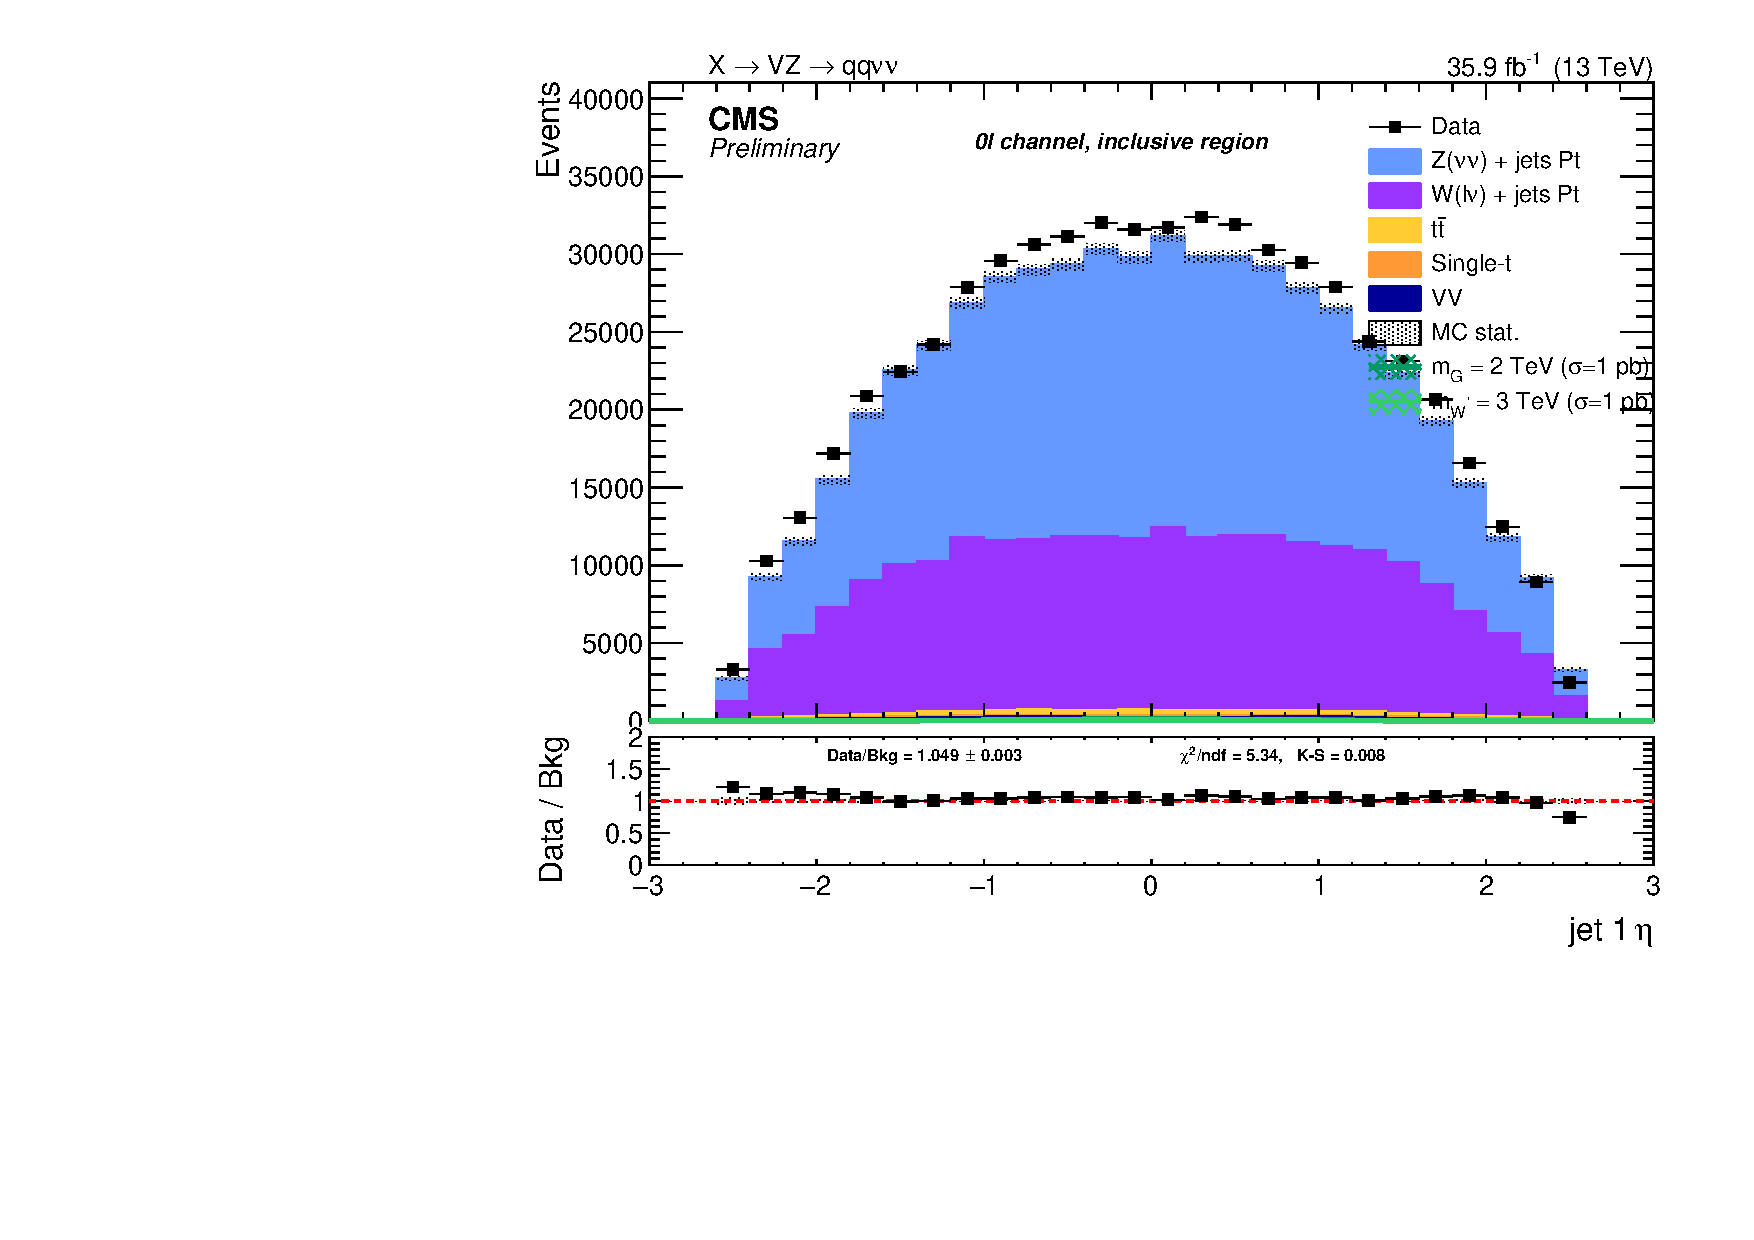
\includegraphics[width=.495\textwidth]{plots/v9_U/XVZnnInc/FatJet1_eta.pdf}
  \end{center}
  \caption{Leading AK8 jet $\eta$ spectra after selections.}
  \label{fig:AK8jet_eta}
\end{figure}


Since it has been measured that the jet energy resolution (JER) is not the same in data and MC, an additional smearing is applied in simulation, in order to get a better agreement, as suggested by JETMET POG~\cite{bib:jetsmear}.

There are two independent ways to get the smearing. With the scaling method, corrected four-momentum of a reconstructed jet is rescaled with a factor
$$c_{\text{JER}} = 1 + (s_{\text{JER}} - 1) \frac{p_T - p_T^{\text{ptcl}}}{p_T},$$
where $p_T$ is its transverse momentum, $p_T^{\text{ptcl}}$ is the transverse momentum of the corresponding jet clustered from generator-level particles, and $s_{\text{JER}}$ is the data-to-simulation core resolution scale factor. Factor $c_{\text{JER}}$ is truncated at zero, i.e. if it is negative, it is set to zero.
This method only works if a well-matched particle-level jet is present and can result in a large shift of the response otherwise. The following requirements are imposed for the matching:
$$\Delta R < R_{\text{cone}} / 2, |p_T - p_T^{\text{ptcl}}| < 3 \sigma_{\text{JER}} p_{T}.$$
Here $R_{\text{cone}}$ is the jet cone size parameter (for instance, 0.4 for AK4 jets) and $\sigma_{\text{JER}}$ is the relative \pt resolution as measured in simulation.

An alternative approach, which does not require the presence of a matching particle-level jet, is the stochastic smearing. In this case corrected jet four-momentum is rescaled with a factor $$c_{\text{JER}} = 1 + \mathcal{N}(0, \sigma_{\text{JER}}) \sqrt{max(s_{\text{JER}}^2 - 1, 0)},$$ where $\sigma_{\text{JER}}$ and $s_{\text{JER}}$ are the relative \pt resolution in simulation and data-to-simulation scale factors, and $\mathcal{N}(0, \sigma)$ denotes a random number sampled from a normal distribution with a zero mean and variance $\sigma^2$. As before, scaling factor $c_{\text{JER}}$ is truncated at zero. This method only allows to degrade the resolution.

The smearing procedure adopted in this analysis is the hybrid method: when matching particle-level jet is found, the scaling method is used; otherwise the stochastic smearing is applied. The smearing coefficients and their errors, provided by JETMET POG, are reported in Tab.~\ref{tab:smear} for 2016 data (tag: {\tt Spring1625nsV10}).

\begin{table}[!htb]
  \centering
  \begin{tabular}{l|ccccccc}
    Jet $\eta$ & SF \\
    \hline
    $0.0-0.5$ & $1.109 \pm 0.008$ \\
    $0.5-0.8$ & $1.138 \pm 0.013$ \\
    $0.8-1.1$ & $1.114 \pm 0.013$ \\
    $1.1-1.3$ & $1.123 \pm 0.024$ \\
    $1.3-1.7$ & $1.084 \pm 0.011$ \\
    $1.7-1.9$ & $1.084 \pm 0.011$ \\
    $1.9-2.1$ & $1.140 \pm 0.047$ \\
    $2.1-2.3$ & $1.067 \pm 0.053$ \\
    $2.3-2.5$ & $1.177 \pm 0.041$ \\
    $2.5-2.8$ & $1.364 \pm 0.039$ \\
    $2.8-3.0$ & $1.857 \pm 0.071$ \\
    $3.0-3.2$ & $1.328 \pm 0.022$ \\
    $3.2-5.0$ & $1.16  \pm 0.029$ \\
  \end{tabular}
  
  \caption{Smearing coefficients and JER uncertainties.}
  \label{tab:smear}
\end{table}

\clearpage
\subsection{Jet mass}\label{ssec:jetmass}

The jet mass is the main observable in distinguishing a V-jet from a QCD jet. Jet grooming consists in the suppression of uncorrelated UE/PU (underlying event and pile-up) radiation from the target jet and improves the discrimination pushing the jet mass for QCD jets towards lower values while maintaining the jet mass for V-jets around the boson-mass.

%Two different grooming algorithms were originally considered:
The grooming algorithm considered in this analysis is the following:
\begin{itemize}
%%  \item[\bf{Trimming}:] Trimming is a technique that ignores regions within a jet that falls below a minimum \pt threshold. Trimming reclusters the jet's constituents with a radius $R_{sub}$ and then accepts only the subjets that have $p_{T,sub} > f_{cut}$, where $f_{cut}$ is typically taken proportional to \HT , the scalar sum of the \pt of all jet reconstructed in the event.
%%  \item[\bf{Filtering}:] This procedure provides a hierarchical structure for the clustering like the \kt algorithm, but in angles rather than in relative transverse momenta. It creates a series of n new subjects $s_1, s_2, \dots s_n$ ordered in descending \pt. The final jet is redefined as the sum of the four-momenta of the three highest \pt subjets $\sum_i^{min(n,3)} s_i$.
%  \item[\bf{Pruning}:] The idea is to take a jet of interest and then to recluster it using a vetoed sequential clustering algorithm. Clustering is performed with the CA algorithm, but particles are discarded if they are too far away in $\Delta R$: 
% %\begin{linenomath}\begin{equation}
% $$ \Delta R_{ij} > D_{cut} \alpha \frac{m_j}{p_{T,j}}$$
% %\end{equation}\end{linenomath}
%  and the energy sharing is too asymmetric: 
% % \begin{linenomath}\begin{equation}
% $$ z_{ij} = \frac{min(p_{T,i}, p_{T,j})}{p_{T,i+j}} < z_{cut} $$
% % \end{equation}\end{linenomath}
%  where $z_{cut}$ and $\alpha$ are parameters of the algorithm. If both these conditions are satisfied the softer of the two particles is not considered.
  \item[\bf{Soft-drop}:] The ``soft drop declustering'' is a jet substructure technique which recursively removes soft wide-angle radiation from a jet~\cite{Larkoski:2014wba}. The soft drop algorithm depends on two parameters: a soft threshold $z$ cut and an angular exponent $\beta$. Like any grooming method, soft drop declustering removes wide-angle soft radiation from a jet in order to mitigate the effects of contamination from initial state radiation (ISR), underlying event (UE), and multiple hadron scattering (pileup). Given a jet of radius $R_0$ with only two constituents, the soft drop procedure removes the softer constituent unless:
%\begin{linenomath}\begin{equation}
 $$\frac{\min(\pt^1,\pt^2)}{\pt^1+\pt^2} > z_{cut} \left( \frac{\Delta R_{12}}{R_0} \right)^\beta$$
%\end{equation}\end{linenomath}
By construction, this condition fail for wide-angle soft radiation. The degree of jet grooming is controlled by $z_{cut}$ and $\beta$, with $\beta \to \infty$ returning back an ungroomed jet.  The $\beta=0$ limit of the energy loss is particularly interesting, since it is largely insensitive to the value of the strong coupling constant. The default parameters used by CMS are $\beta=0$ and $z_{cut}=0.1$.
\end{itemize}

%In general, the filtering algorithm is the least aggressive grooming technique, with groomed jet masses close to the original case. The trimming algorithm is moderately aggressive and produces a much wider final mass distribution. Pruning is the most aggressive technique and a bimodal distribution begins to appear: in cases where the pruned jet mass is small, jets usually have most of their energy configured in core components with little gluon radiation, which leads to narrow jets. Instead, when the pruned jet mass is large, the jets are split more symmetrically.

The grooming algorithm, {\bf soft-drop}, is used in association with {\bf PUPPI} in order to remove soft and wide-angle radiations and the pile-up contribution. It is a shared choice among all the diboson analyses, praised by theoreticians.

Unfortunately, the default soft-drop + PUPPI jet mass suffers from a systematic shift from the expected value of about $\sim 10\%$, and some residual dependence on the jet \pt. Further corrections to the jet mass have been applied:

\begin{enumerate}
  \item[{\bf Gen}:] a \pt-dependent correction to account for a small shift in the generated vector boson mass, applied only on simulated samples
  \item[{\bf Reco}:] a \pt-dependent correction to the reconstructed jet mass, applied separately for jets in the barrel and endcaps regions
\end{enumerate}

These corrections are evaluated centrally by JMAR and documented in~\cite{AN-16-215}, and applied accordingly within the analysis.

Figure~\ref{fig:fatjet_pre_softdroppuppimass_ZZ}-~\ref{fig:fatjet_softdroppuppimass} show the jet mass for \PW or \Z bosons before and after the correction, without applying any cut on this variable.

\begin{figure}[!htb]
  \begin{center}
    %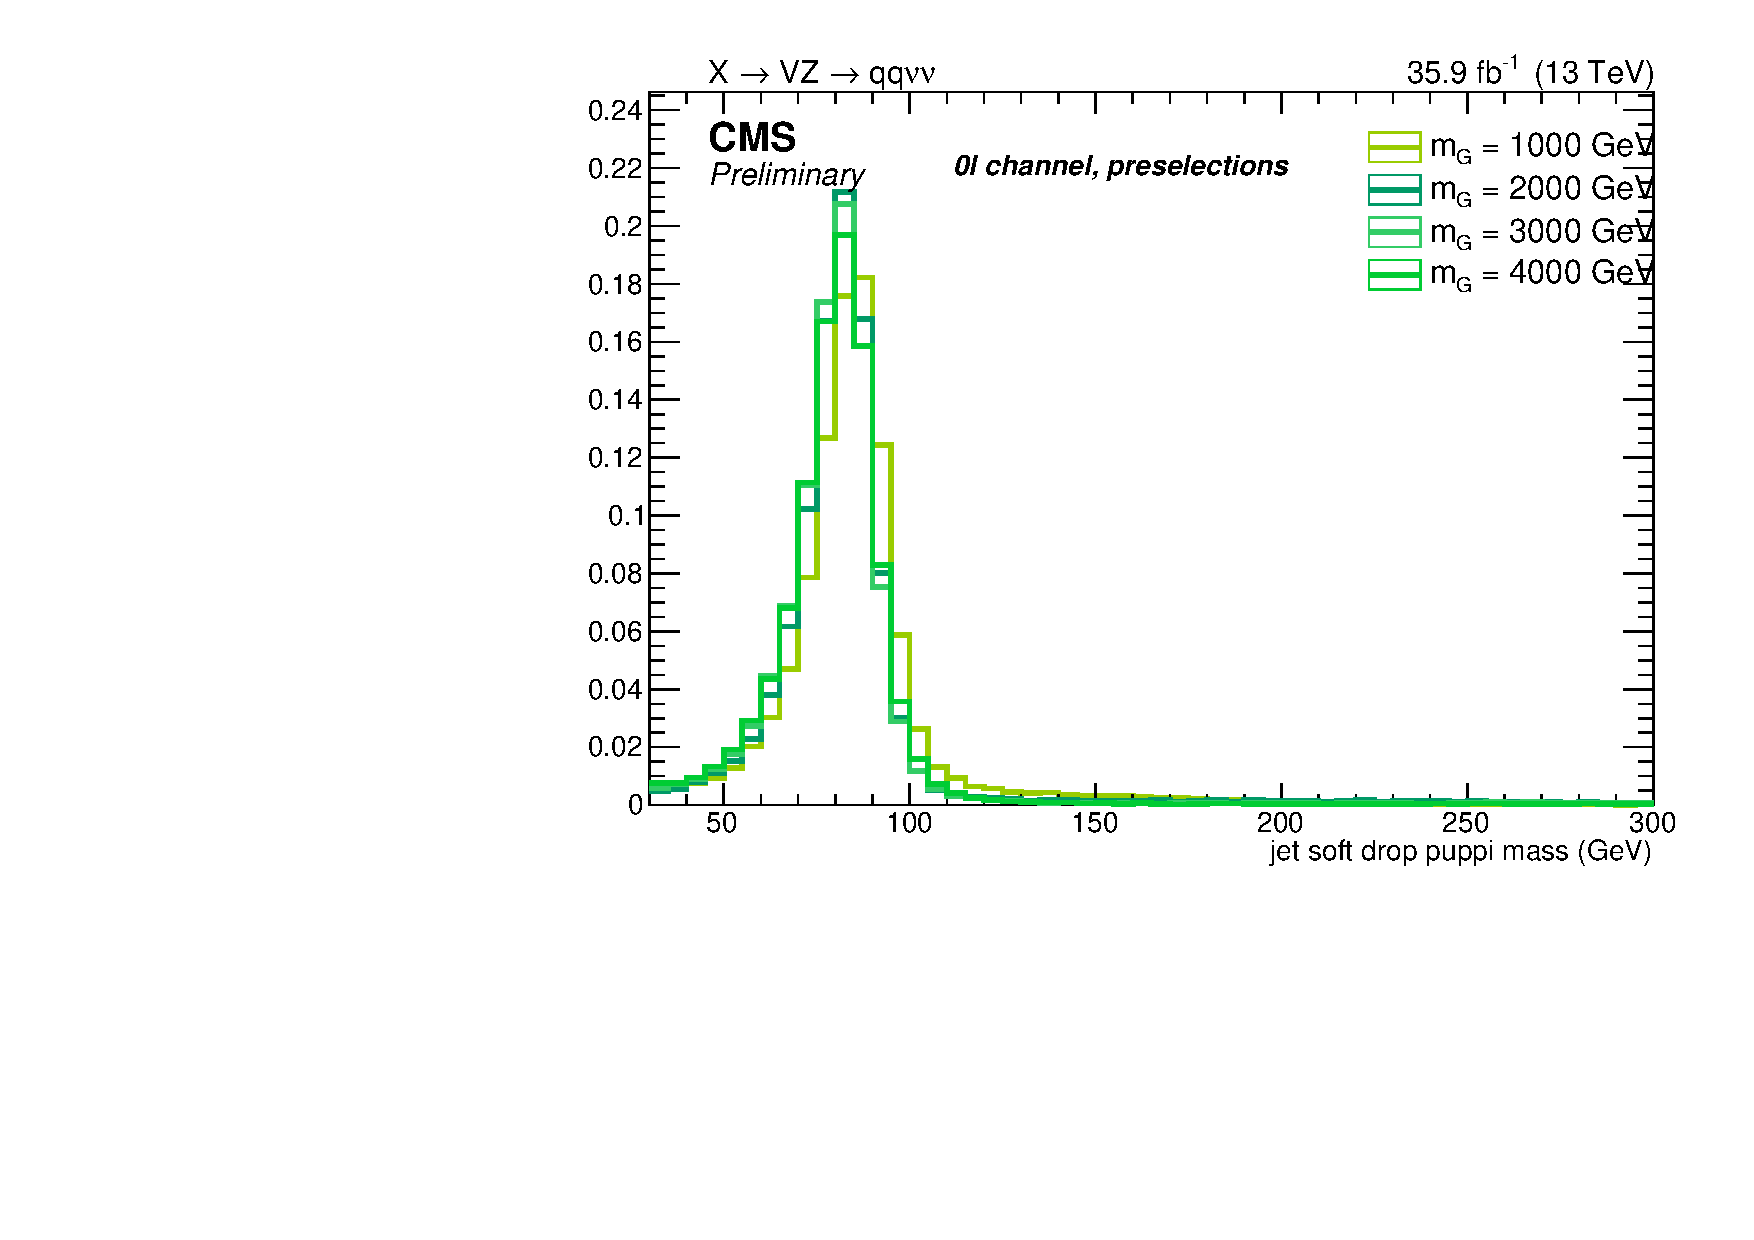
\includegraphics[width=.495\textwidth]{plots/v9/XVZnnPre/FatJet1_softdropPuppiMass_signalZZ.pdf}
    %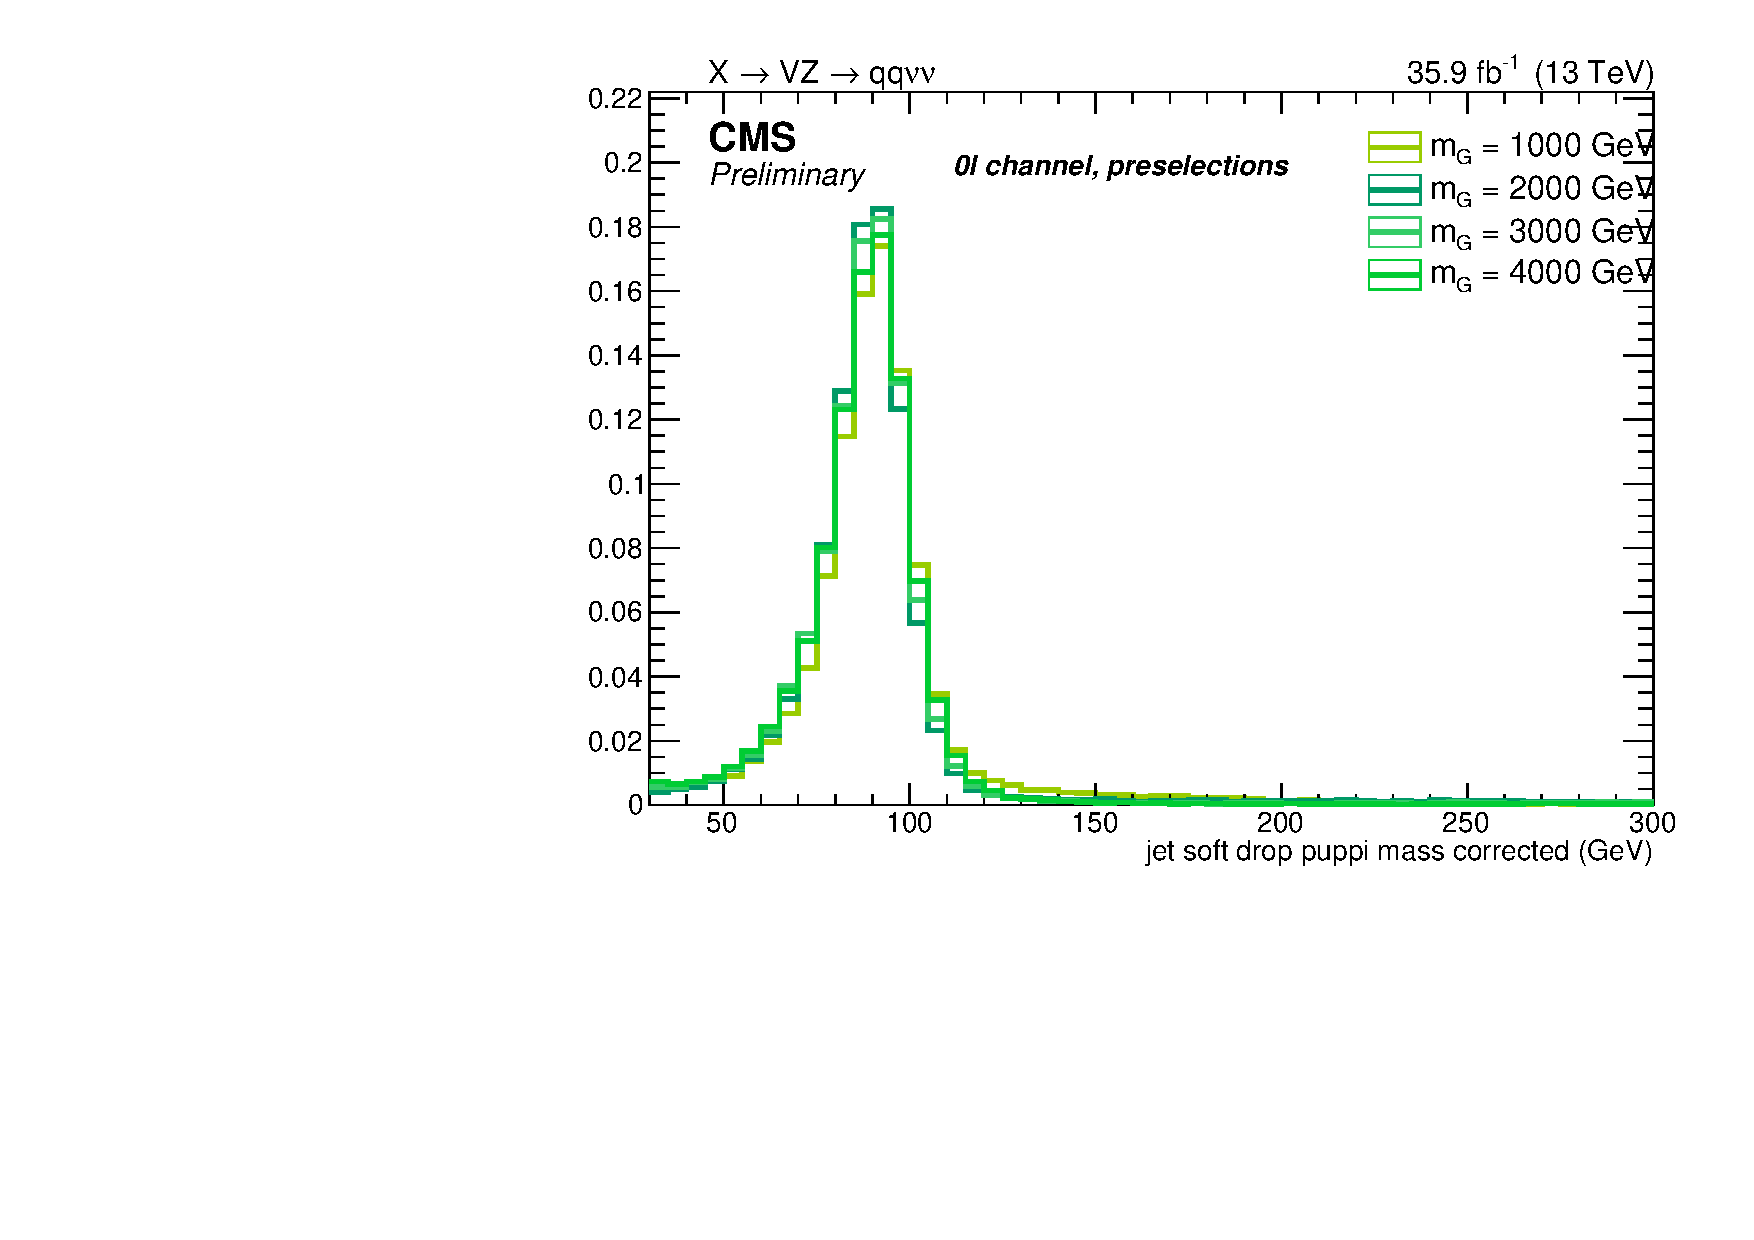
\includegraphics[width=.495\textwidth]{plots/v9/XVZnnPre/FatJet1_softdropPuppiMassCorr_signalZZ.pdf}
  \end{center}
  \caption{Softdrop + PUPPI mass of AK8 jet reconstructed for different bulk graviton signal samples; left: before corrections. right: after corrections.}
  \label{fig:fatjet_pre_softdroppuppimass_ZZ}
\end{figure}

\begin{figure}[!htb]
  \begin{center}
    %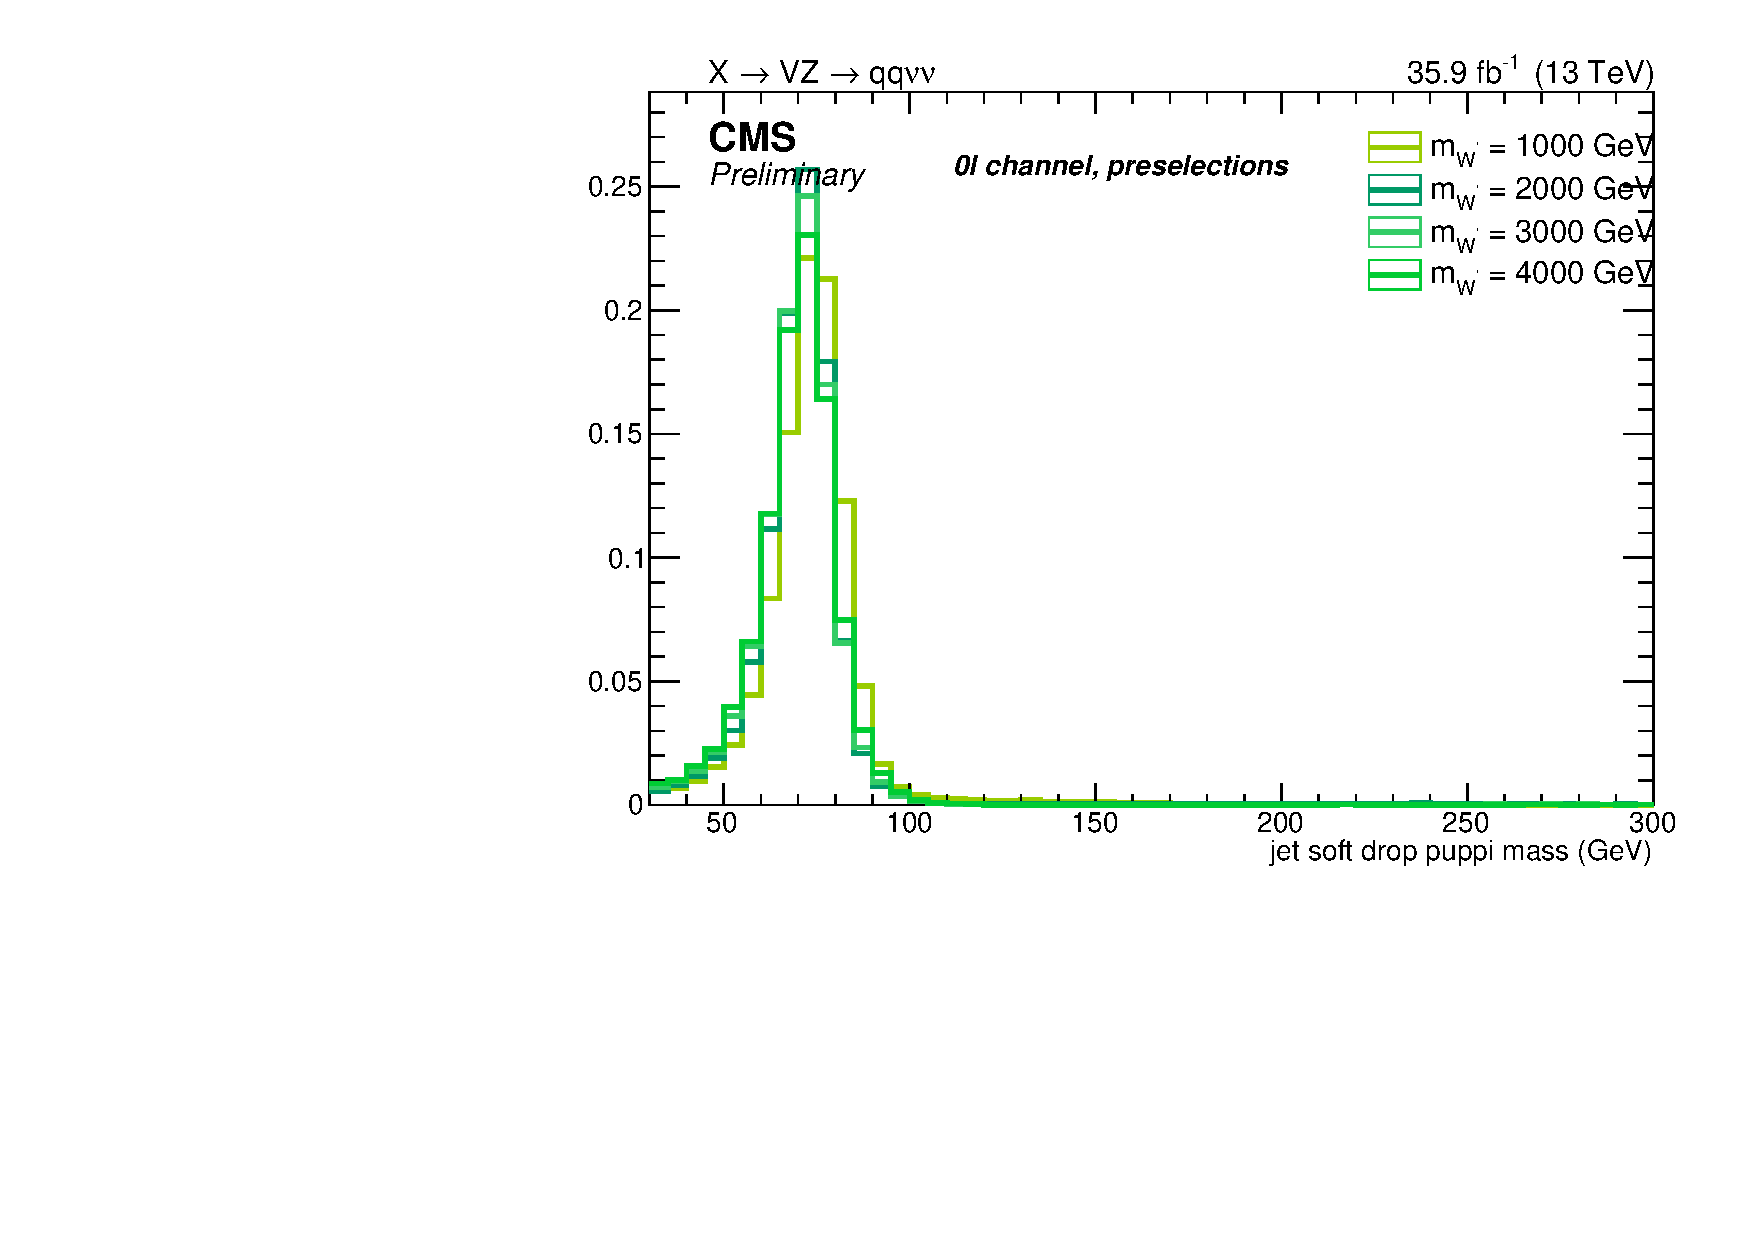
\includegraphics[width=.495\textwidth]{plots/v9/XVZnnPre/FatJet1_softdropPuppiMass_signalWZ.pdf}
    %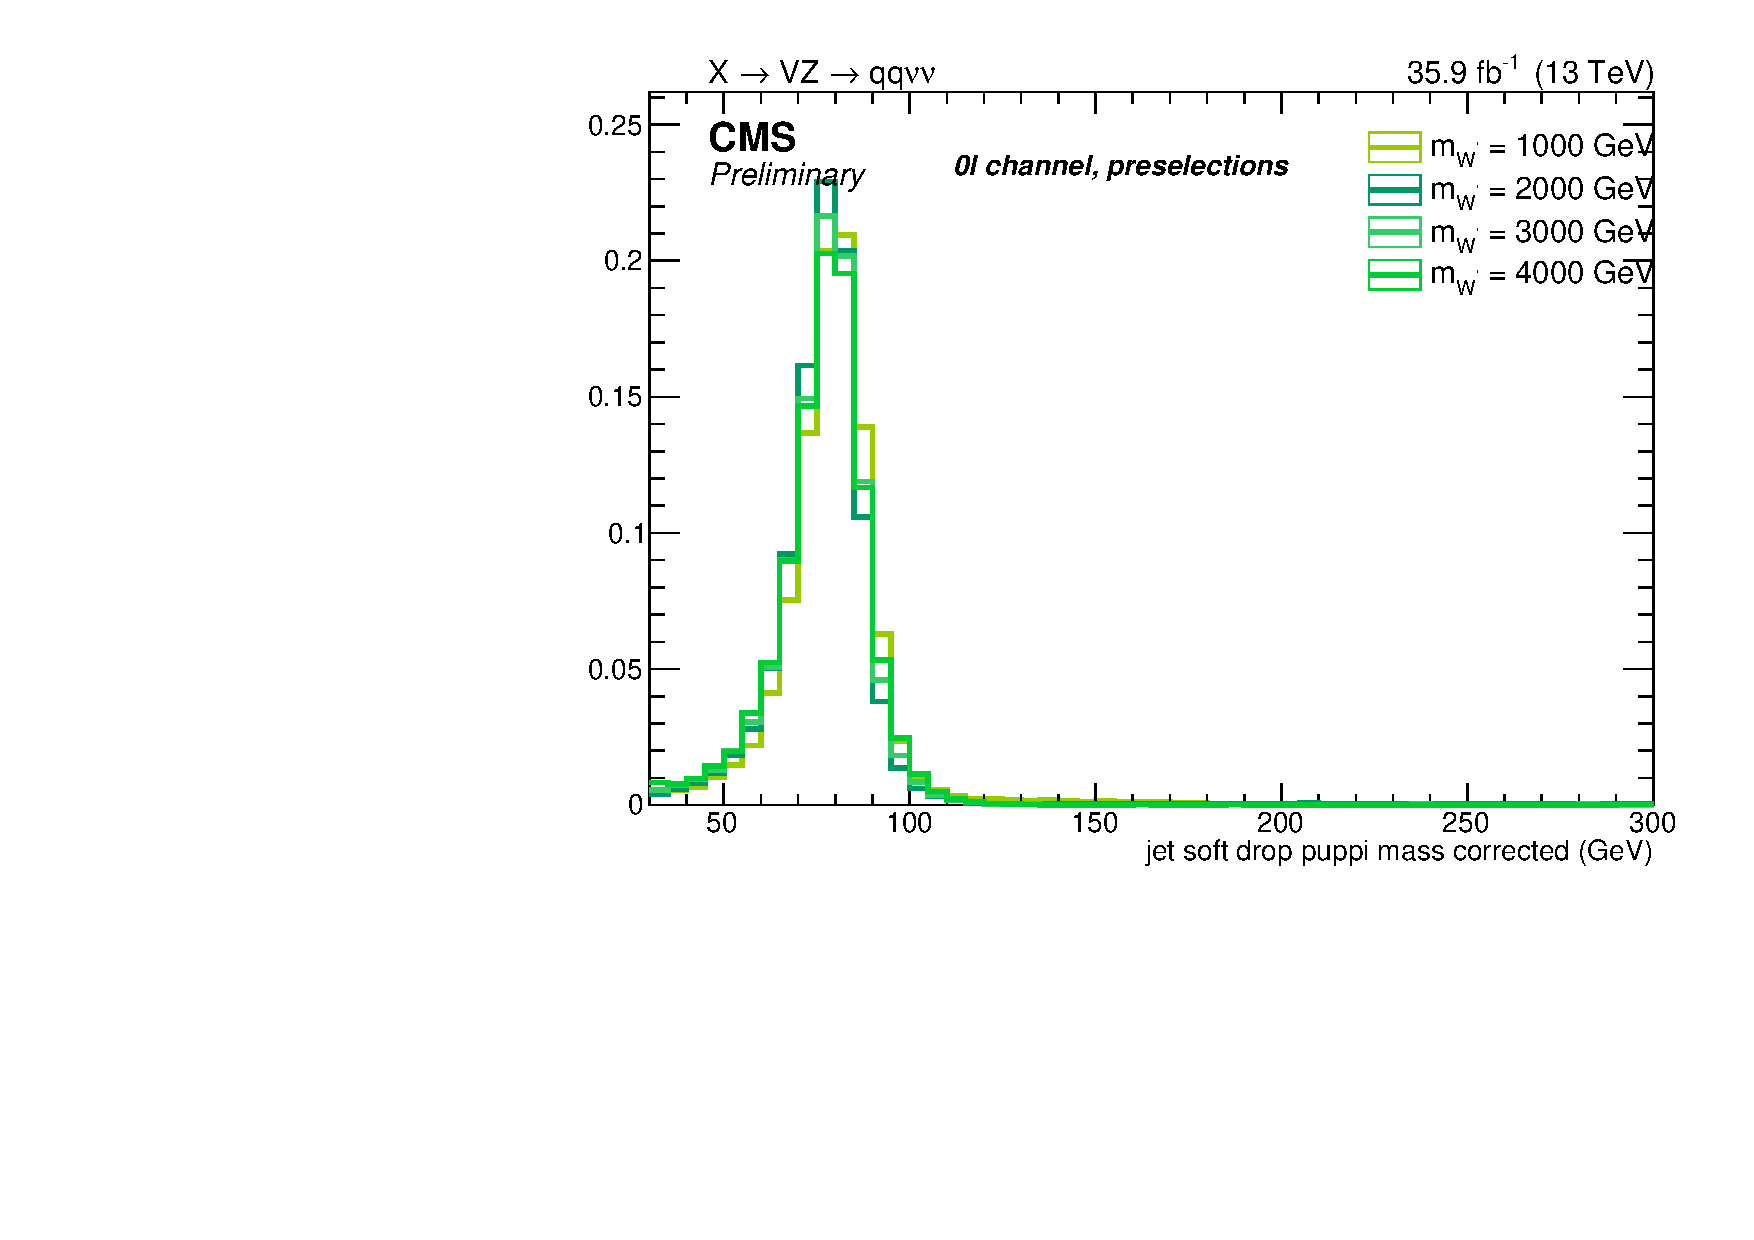
\includegraphics[width=.495\textwidth]{plots/v9/XVZnnPre/FatJet1_softdropPuppiMassCorr_signalWZ.pdf}
  \end{center}
  \caption{Softdrop + PUPPI mass of AK8 jet reconstructed for different $W^{'}$ signal samples; left: before corrections. right: after corrections.}
  \label{fig:fatjet_pre_softdroppuppimass_ZZ}
\end{figure}

\begin{figure}[!htb]
  \begin{center}
    %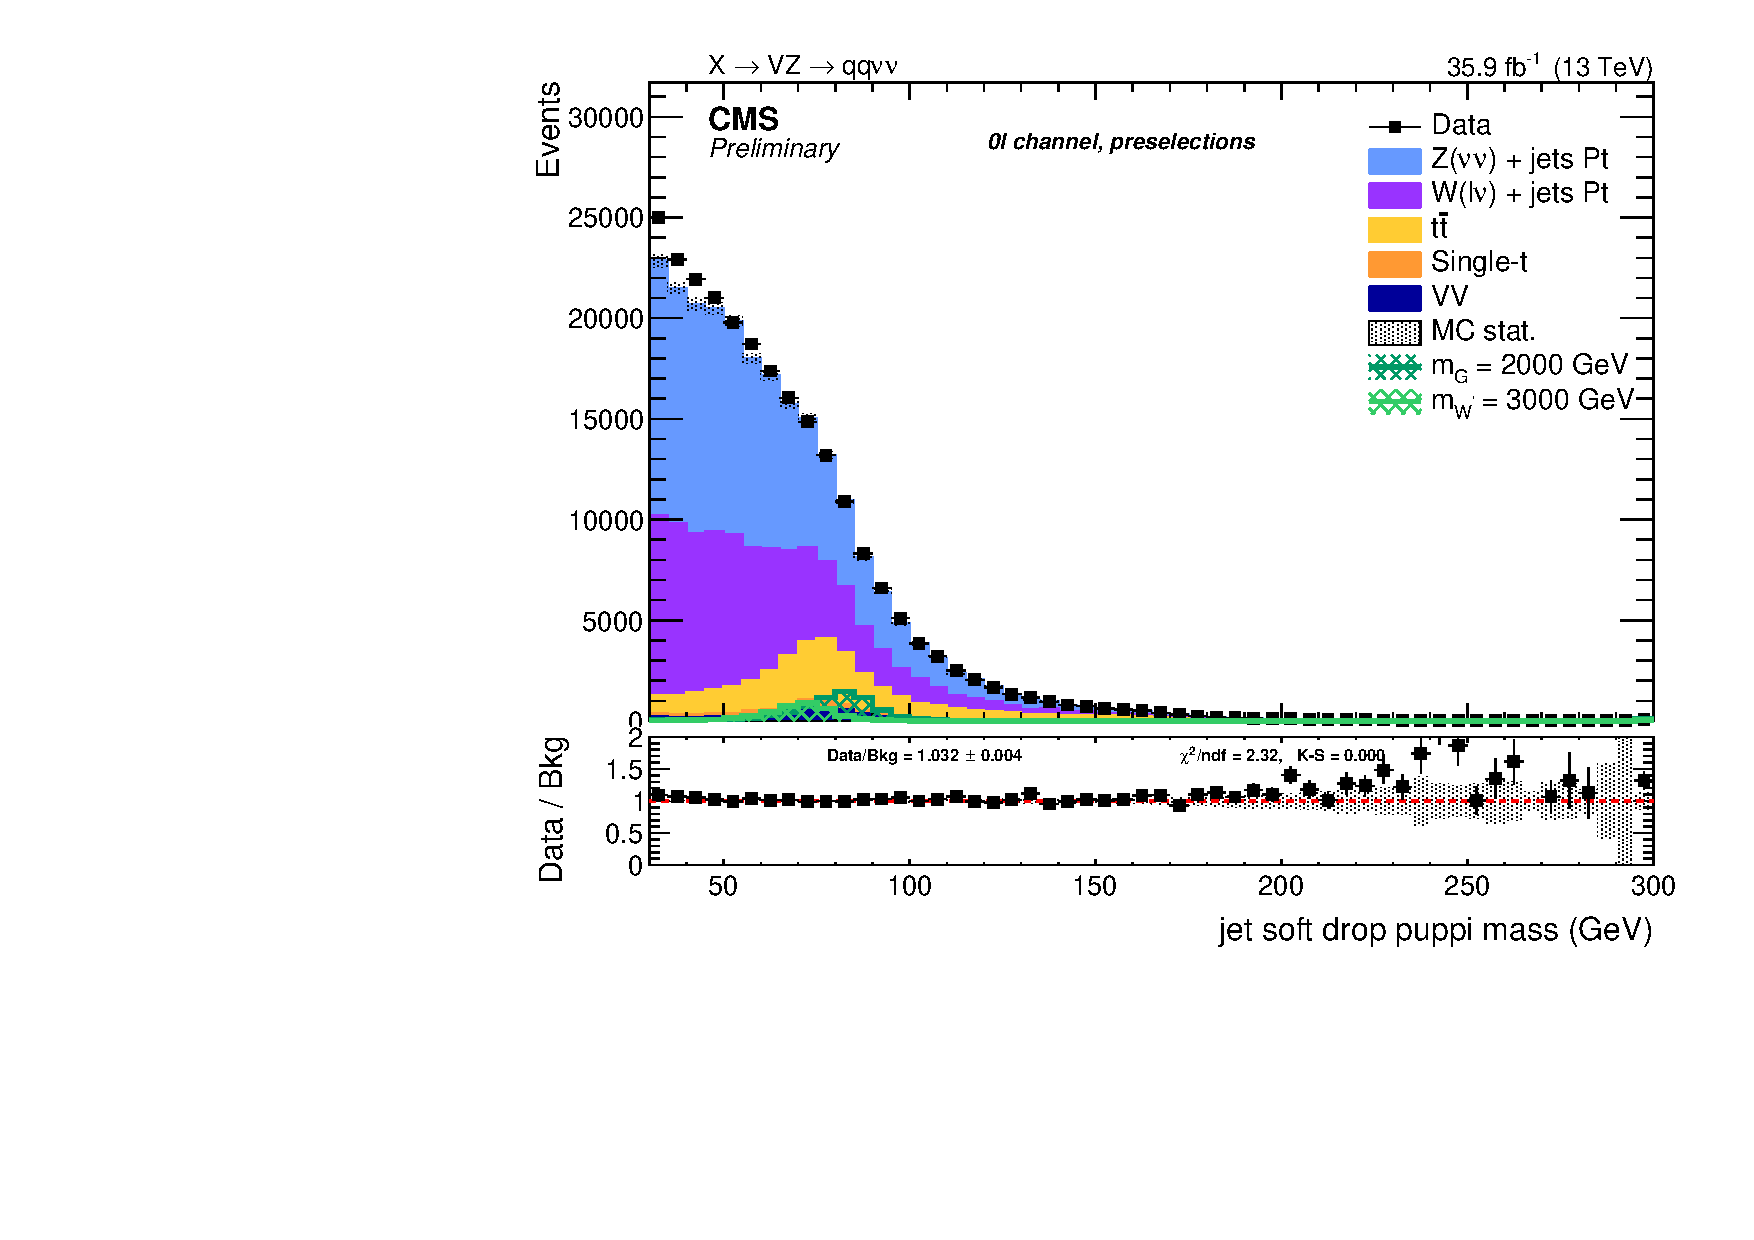
\includegraphics[width=.495\textwidth]{plots/v9/XVZnnPre/FatJet1_softdropPuppiMass.pdf}
    %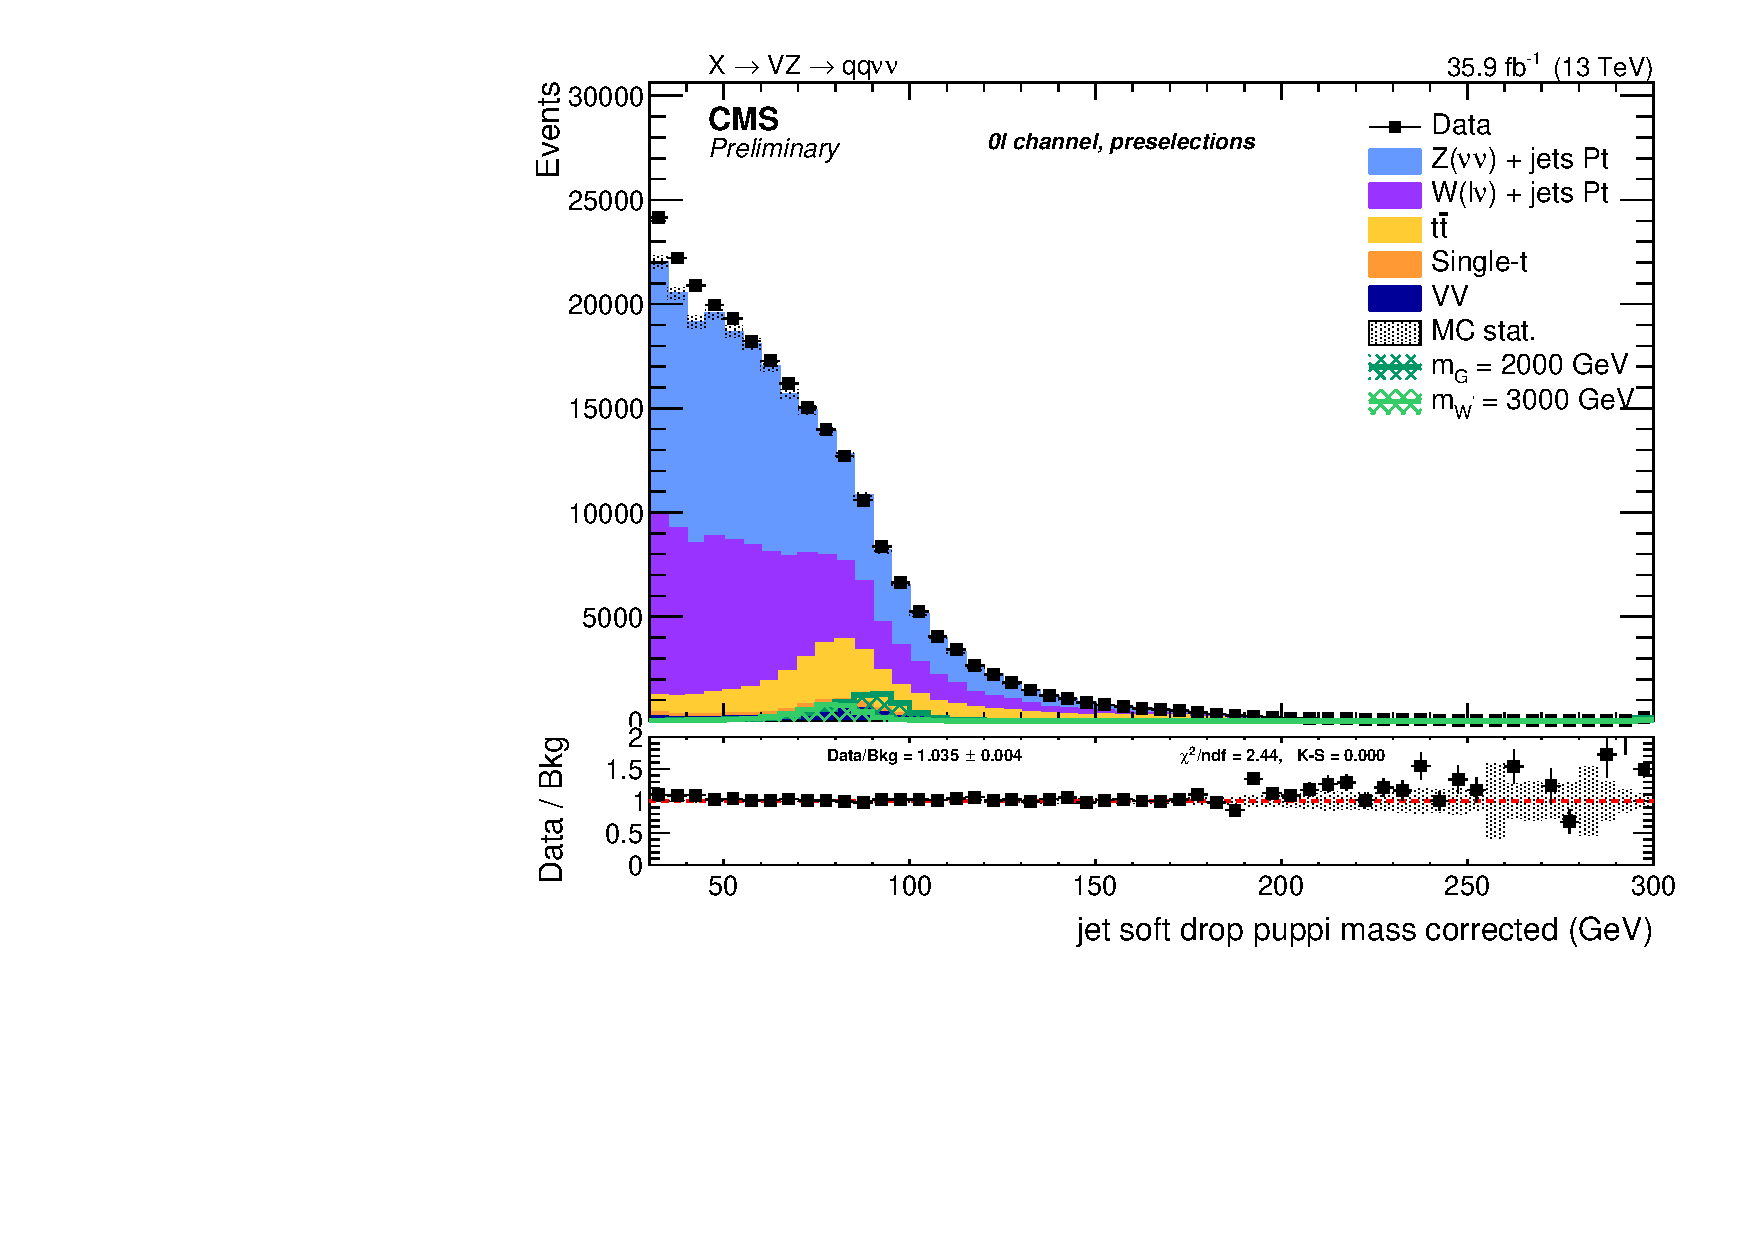
\includegraphics[width=.495\textwidth]{plots/v9/XVZnnPre/FatJet1_softdropPuppiMassCorr.pdf}
  \end{center}
  \caption{Softdrop + PUPPI mass of AK8 jet; left: before corrections. right: after corrections.}
  \label{fig:fatjet_softdroppuppimass}
\end{figure}

Furthermore, in order to obtain a better data-Monte Carlo agreement, a smearing procedure has been applied to the puppi softdrop mass, by using the stochastic method, with a constant smearing coefficent provided by JETMET POG ($1.00 \pm 0.20$), that does not depend on jet pseudorapidity if it is restricted to $|\eta|<2.5$.

%\clearpage
\subsection{Jet substructure}\label{ssec:jetsub}

In order to further discriminate signal from background, it useful to investigate the inner structure of the jet. Studying the distribution of the jet constituents with respect to the jet axis allows us to test the hypothesis of the existence of multiple substructures, that could be evidence of jets originated by more than one parton. This procedure proceeds as follows: the constituents of the jet are clustered again with the $k_T$ algorithm, however the procedure is stopped when one obtains N subjets. 
Then, a new variable, the N-subjectiness, is introduced. It is defined as:
%\begin{linenomath}\begin{equation}
$$\tau_N = \frac{1}{d_0} \sum_k p_{T,k} min( \Delta R_{1,k}^\beta, \Delta R_{2,k}^\beta, \dots, \Delta R_{N,k}^\beta )$$
%\end{equation}\end{linenomath}
where $\beta$ is an arbitrary parameter, the index $k$ runs over the jet constituents and the distances $\Delta R_{N,k}$ are calculated with respect to the axis of the N-th subjet, obtained by one iteration of $\tau$ minimization by varying the subjet axes around the $k_T$ subjet axes.

The normalization factor $d_0$ is calculated as $d_0 = \sum_k p_{T, k} R_0^\beta$, setting $R_0$ to the radius of the original jet.
The N-subjettiness is always included in the interval from 0 to 1 and represents the compatibility of the jet structure with an N-subjet hypothesis: small values correspond to high compatibility. Indeed, $\tau_N$ weights the transverse momentum of the jet constituents by their angular distance to the closest subjet.
In this analysis the N-subjettiness is calculated from the ungroomed jet with the parameter $\beta=1$. The subjettiness related to the one and two subjet hypothesis is thus:
%\begin{linenomath}\begin{equation}
$$\tau_1 = \frac{1}{d_0} \sum_k p_{T,k} \Delta R_{1,k}$$
%\end{equation}\end{linenomath}
and
%\begin{linenomath}\begin{equation}
$$\tau_2 = \frac{1}{d_0} \sum_k p_{T,k} min( \Delta R_{1,k}, \Delta R_{2,k} )$$
%\end{equation}\end{linenomath}
In principle, these two quantities should allow us to distinguish the dipole-like
nature of the showering of the Higgs decay from the classic monopole structure of
QCD jets. In particular, the variable that best discriminates between V-jets and
QCD jets is the ratio of 2-subjettiness and 1-subjettiness, $\tau_{21} = \tau_2 / \tau_1$.

Figure~\ref{fig:fatjet_pre_tau21} shows the $\tau_{21}$ distributions for the PUPPI algorithm.

\begin{figure}[!htb]
  \begin{center}
    %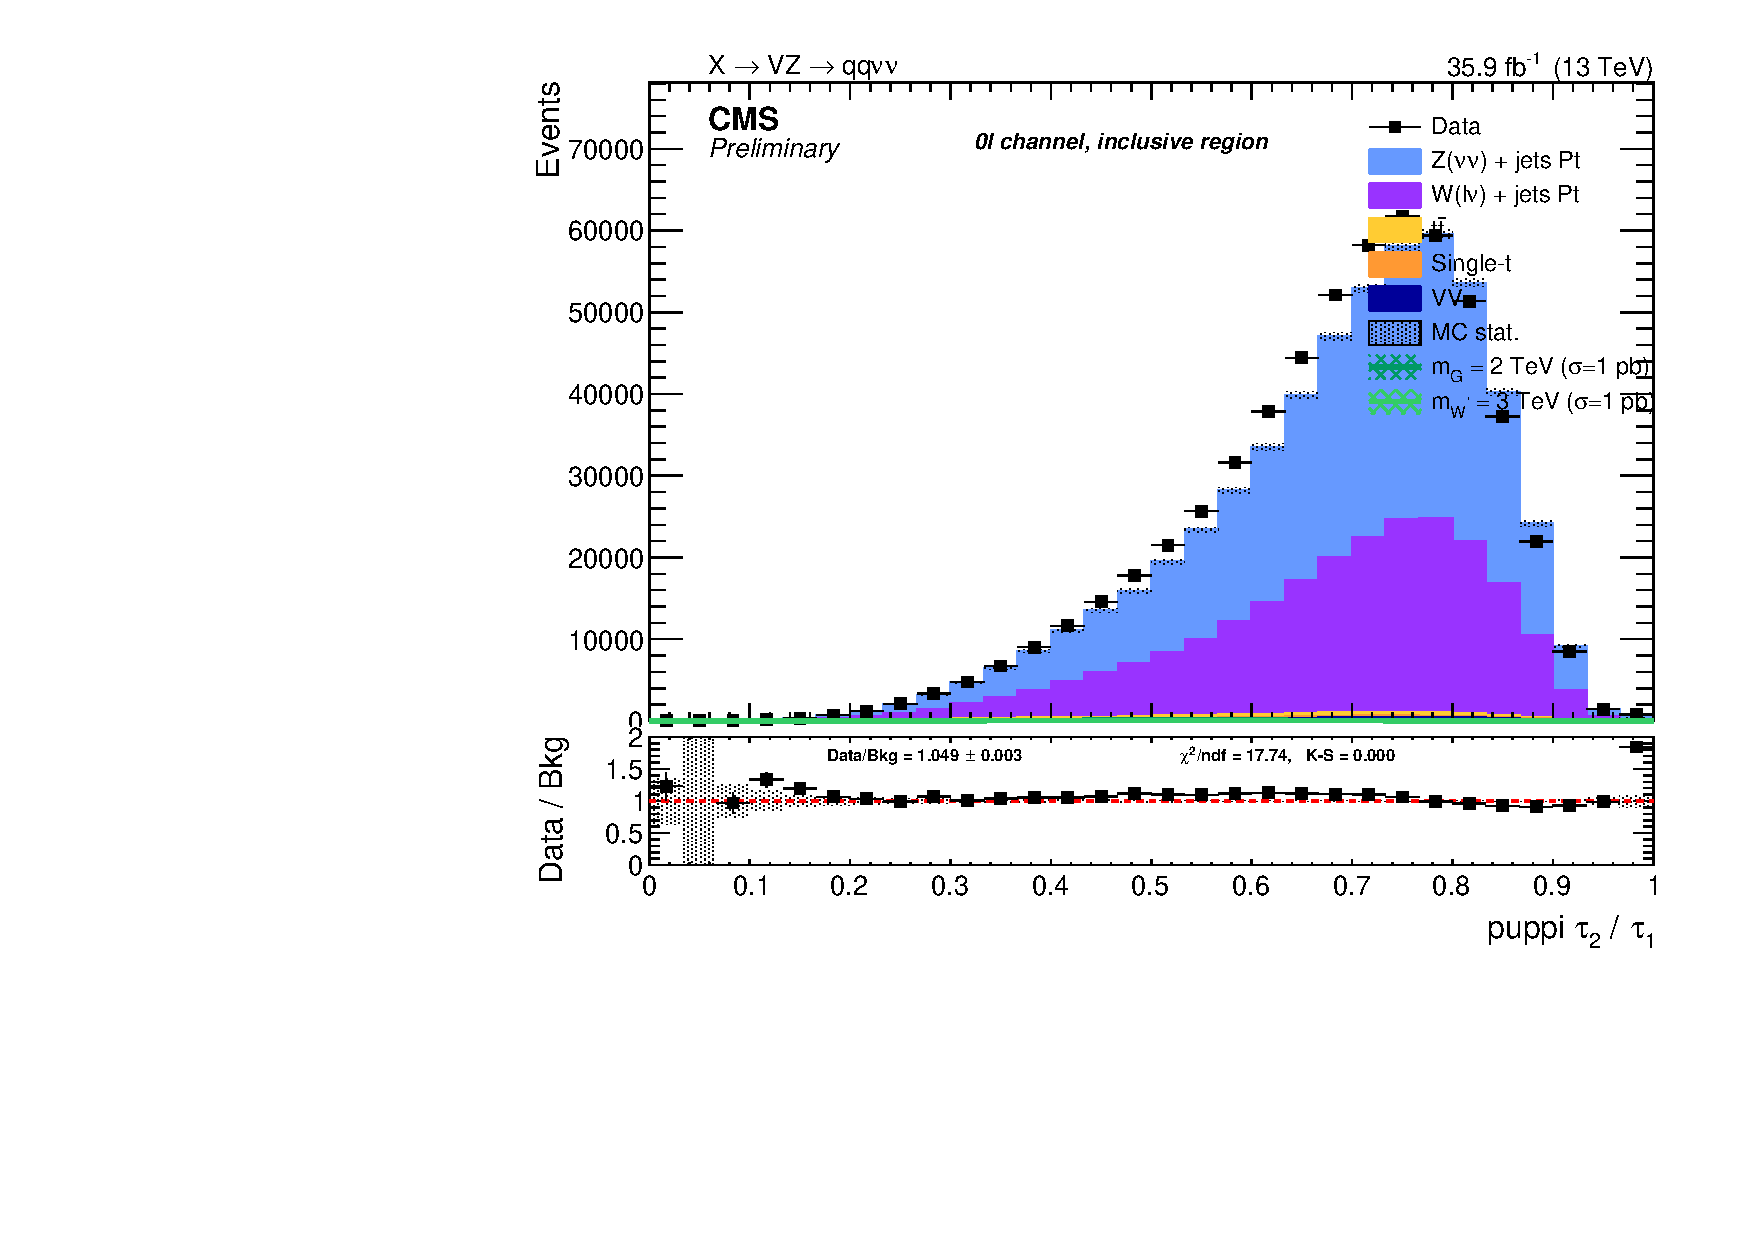
\includegraphics[width=.495\textwidth]{plots/v9_U/XVZnnInc/FatJet1_puppiTau21.pdf}
  \end{center}
  \caption{$\tau_{21}$ subjettiness of PUPPI AK8 jet after inclusive selections.}
  \label{fig:fatjet_pre_tau21}
\end{figure}



\section{b-tagging}\label{ssec:btagging}
 
%The presence of a pair of b-quarks from the $\htobb$ decay is a very distinctive signature that permits a strong discrimination against all the backgrounds that involve jets with light flavors. The only  background which cannot be reduced with this technique is the $\Z$ production in association with one or two b-quarks, and the $\Z \to \bbbar$ decay which is also topologically similar to the signal. The latter can be only reduced by applying a jet mass cut, as described in Section~\ref{ssec:jetmass}.
% 
%Tagging b-jets in boosted topologies has been undergone several modifications with respect to Run-I taggers. 
% One of the most important differences is that the tagger algorithms are not directly based on tracks. 
%%Run-II b-taggers are by default applied on the same charged particle-flow candidate list that is used in the jet clustering (\emph{explicit jet-to-track association}). This procedure is applied to subjets as well: b-tagging algorithms are applied to both the fat-jet and the sub-jets, independently. Furthermore, thanks to the explicit jet-to-track association, the two sub-jets do not share any PF-constituent, avoiding unintended correlations.
B-tagging algorithms are applied to both the fat-jet and the sub-jets, independently. For subjets, run-II taggers are by default applied on the same charged particle-flow candidate list that is used in the jet clustering (\emph{explicit jet-to-track association}). Thanks to the explicit jet-to-track association, the two sub-jets do not share any PF-constituent, avoiding unintended correlations.
% 
% 
%Several algorithms have been developed to tag jets from b-quarks. The recommended and best-performing algorithm is the {\tt pfCombinedInclusiveSecondaryVertexV2BJetTags}, often shortened to \emph{combined secondary vertex (CSV)}. This algorithm involves the use of secondary vertices, together with other lifetime information, like the IP significance or decay lengths. Secondary vertices are reconstructed with the inclusive vertex finder algorithm, that does not require jets (and thus is independent on the jet size) and uses all tracks to reconstruct secondary vertices~\cite{cms:JHEP032011136}. %In order to provide discrimination even when no secondary vertices are found, so the maximum possible b-tagging efficiency is not limited by the secondary vertex reconstruction efficiency ($50 \sim 60\%$). In many cases, tracks with an IP significance $> 2$ can be combined in a so-called pseudo vertex, allowing for the computation of a subset of secondary vertex based quantities even without an actual vertex fit. When even this is not possible, a no vertex category reverts simply to track based variables similarly to the jet probability algorithm. %The list of variables fed as input to an Artificial Neural Network is:
% \begin{itemize}
%   \item  the vertex category (real, pseudo, or no vertex)
%   \item  2D flight distance significance
%   \item  vertex mass
%   \item  number of tracks at the vertex
%   \item  ratio of the energy carried by tracks at the vertex with respect to all tracks in the jet
%   \item  the pseudo-rapidity of the tracks at the vertex with respect to the jet axis
%   \item  2D IP significance of the first track that raises the invariant mass above the charm threshold of 1.5 \GeV when subsequently summing up tracks ordered by decreasing IP significance
%   \item  3D signed IP significances for all tracks in the jet
%   \item  number of tracks in the jet
%   \item  $\Delta R$ between the secondary vertex flight direction and the jet axis
%   \item  number of secondary vertices associated to the jet or sub-jet
% \end{itemize}
 
The jet or sub-jet is considered as tagged if the discriminator value is above some threshold value, often referred to as the cut value, and the efficiency is defined as the number of jets which have a discriminator value that is above that cut divided by the total number of jets (of the same flavor).
% %In other words, the integral of the histogram from a certain discriminator cut up to infinity divided by the total number of jets.
%The typical b-tagging efficiency is between 40\% and 70\% while keeping the rate of mis-identified light-flavor jets between 0.1\% and 10\%. Three working points are usually defined for each algorithm, defining cuts in the discriminators based on the level of mis-tagging. The cut values and the corresponding mis-tagging for light-flavor jets relative to the CSV algorithm are reported in Table~\ref{tab:csvwp}.
% 
% \begin{table}[!htb]
%   \begin{center}
%   \begin{tabular}{lcc}
%   Working point & Cut & $\varepsilon_{light}$\\
%   \hline
%    Loose & 0.605  & $\sim 10\%$ \\
%    Medium & 0.890  & $\sim 1\%$ \\
%    Tight & 0.970  & $\sim 0.1\%$ \\
%   \end{tabular}
%   \end{center}
%   \caption{CSV official working points.}
%   \label{tab:csvwp}
% \end{table}

The b-tagging algorithm used to set the analysis strategy is the Combined Secondary Vertex (CSV)~\cite{bib:btag} discriminator (full name {\tt pfCombinedInclusiveSecondaryVertexV2BJetTags}). Different working points are provided by the POG for Run2 analyses~\cite{BTVPOG}, as shown in table~\ref{tab:btag}, but the only one used in this analysis is the \emph{loose} working point.

\begin{table}[!htb]
  \centering
  \label{tab:btag}
  \begin{tabular}{l|c|c}
     Working point & CSV cut & mis-tag probability\\ 
    \hline
     CSVL (Loose)  & $>0.5426$ & $\approx 10\%$  \\ 
     CSVM (Medium) & $>0.8484$ & $\approx 1\%$   \\ 
     CSVT (Tight)  & $>0.9535$ & $\approx 0.1\%$ \\ 
    \hline
  \end{tabular}
  \caption{Working point for CSV b-tagging algorithm.}
  
\end{table}

B-tagging efficiency is not the same in data and MC. In order to take into account this difference, the BTV POG provides collections of b-tagging scale factors for b-jets and mistagged light jets, measured for different physics processes, for the supported tagging algorithms and the three standard working points~\cite{bib:btag}. A weight is calculated on a per-event basis as a function of the b-tagging status of the jets and their kinematic variables~\cite{bib:btagsf}.%; this is a simple and effective method if there are a small number of possible combinations of jets and b-tagged jets.%Unfortunately, this is not the case of the present analysis. Other techniques allow to take into account the scale factors provided by BTV by \emph{reshaping} the discriminator output; this method has been already successfully applied in the SM VH analysis~\cite{bib:SMVH}, and is also described in detail in Ref.~\cite{bib:AZh,Khachatryan:2015lba}. The reshaping method does not sensibly increase the b-tagging scale factors uncertainty with respect to using single operating point SFs or other techniques used to apply the same scale factors.
% 
% The CSV discriminator output has been reshaped in the simulation taking into account the official SF provided by the POG. The procedure is tested in a \ttbar-enriched sample, obtained by requiring one tight and isolated muon and a tight electron and at least one jet above 30 \GeV. The original and reshaped CSV distribution of the leading  and sub-leading jet in the event are reported in Fig.~\ref{fig:reshaping1} and Fig.~\ref{fig:reshaping2}, respectively for events passing a 0-lepton and 1-electron selections.
% 
% \begin{figure}[!htb]
%   \centering
%     \includegraphics[width=.495\textwidth]{plots/XZhnnInc/bjet1_CSVR.pdf}
%     \includegraphics[width=.495\textwidth]{plots/XZhnnInc/bjet1_CSV.pdf}
%   
%   \caption{Combined Seconday Vertex discriminator before (left) and after (right) the reshaping procedure applied to the highest-CSV AK4 jet in the event in the 0-lepton channel.}
%   \label{fig:reshaping1}
% \end{figure}
% 
% \begin{figure}[!htb]
%   \centering
%     \includegraphics[width=.495\textwidth]{plots/XWhenInc/bjet1_CSV.pdf}
%     \includegraphics[width=.495\textwidth]{plots/XWhenInc/bjet1_CSVR.pdf}
%   \caption{Combined Seconday Vertex discriminator before (left) and after (right) the reshaping procedure applied to the highest-CSV AK4 jet in the event in the 1-electron channel.}
%   \label{fig:reshaping2}
% \end{figure}
% 
% \clearpage

In this analysis, b-tagging is used in order to reject events where a top quark is involved, by asking to the AK4 jets not laying in the AK8 jet cone to be anti b-tagged (in practice, the maximum CSV value allowed is the loose working point, CSVL).

\section{Missing Energy}
{\color{red} How the MET is reconstructed}
 
The \MET is the imbalance in the transverse momentum of all visible particles, and it is reconstructed with the particle flow algorithm~\cite{bib:PF1}. The \emph{raw} \MET is defined as the inverse vectorial sum of the transverse momentum of all the reconstructed charged and neutral particle flow candidates: $\vec{\MET}= - \sum_{i=0}^{all} \vec{\pt}_i$.
The raw \MET is systematically different from true \MET, for many reasons including the non-compensating nature of the calorimeters and detector misalignment. To better estimate the true \MET, corrections can be applied:
\begin{itemize}
   \item[\emph{Type-0}:] a mitigation for the degradation of the \MET reconstruction due to the pileup interactions, by applying the CHS algorithm. However, the \MET contribution from pileup neutral particles cannot be easily subtracted; the assumption is that the \MET contribution term of charged and neutral pileup particles are the same, and cancellation at the true level is exact: $\sum_{neuPU} \vec{\pt}_i^{true} + \sum_{chPU} \vec{\pt}_i^{true} = 0$. An additional \MET term is then added to the raw \MET to take into account the neutral PU contribution, which is equal to the charged one with a multiplicative scale factor taking into account calorimeter mismeasurements of low-\pt energy deposits.
   \item[\emph{Type-1}:] propagation of the jet energy corrections (JEC) to MET. The Type-I correction replaces the vector sum of transverse momenta of particles which can be clustered as jets with the vector sum of the transverse momenta of the jets to which JEC is applied. 
 \end{itemize}
% 
Particle flow \MET with type-1 corrections applied is currently the default one used by CMS physics analyses. Additionaly, some \MET filters have been recommended by JETMET POG for Run2 analyses~\cite{JetMETPOG}, in order to remove events with spurios \MET related to detector noise and bad reconstructions, and they are listed in sec.~\ref{sec:data}.
%\begin{itemize}
%\item {\tt HBHENoiseFilter}
%\item {\tt HBHENoiseIsoFilter}
%\item {\tt EcalDeadCellTriggerPrimitiveFilter}
%\item {\tt goodVertices}
%\item {\tt eeBadScFilter} (not recommended for Monte Carlo, hence not applied)
%\item {\tt globalTightHalo2016Filter}
%\item {\tt BadPFMuonFilter}
%\item {\tt BadChargedCandidateFilter}
%\end{itemize}

%\section{Re-computation of \MET corrections and uncertainties}
Since the \MET corrections and uncertainties depend on the JEC applied, they are re-computed accordingly following the JETMETPOG recommendation:
\begin{verbatim}
from PhysicsTools.PatUtils.tools.runMETCorrectionsAndUncertainties import
runMetCorAndUncFromMiniAOD
# If you only want to re-correct and get the proper uncertainties
runMetCorAndUncFromMiniAOD(process,
                           isData=True (or False),
                           )
process.p = cms.Path(process.fullPatMetSequence *
   process.yourAnalyzer)

cms.InputTag("slimmedMETs","","YourProcessName")
\end{verbatim}

Figure~\ref{fig:type1_met} show the \MET distribution for data and Monte Carlo after the corrections and filters.
 
 \begin{figure}[!htb]
   \centering
     %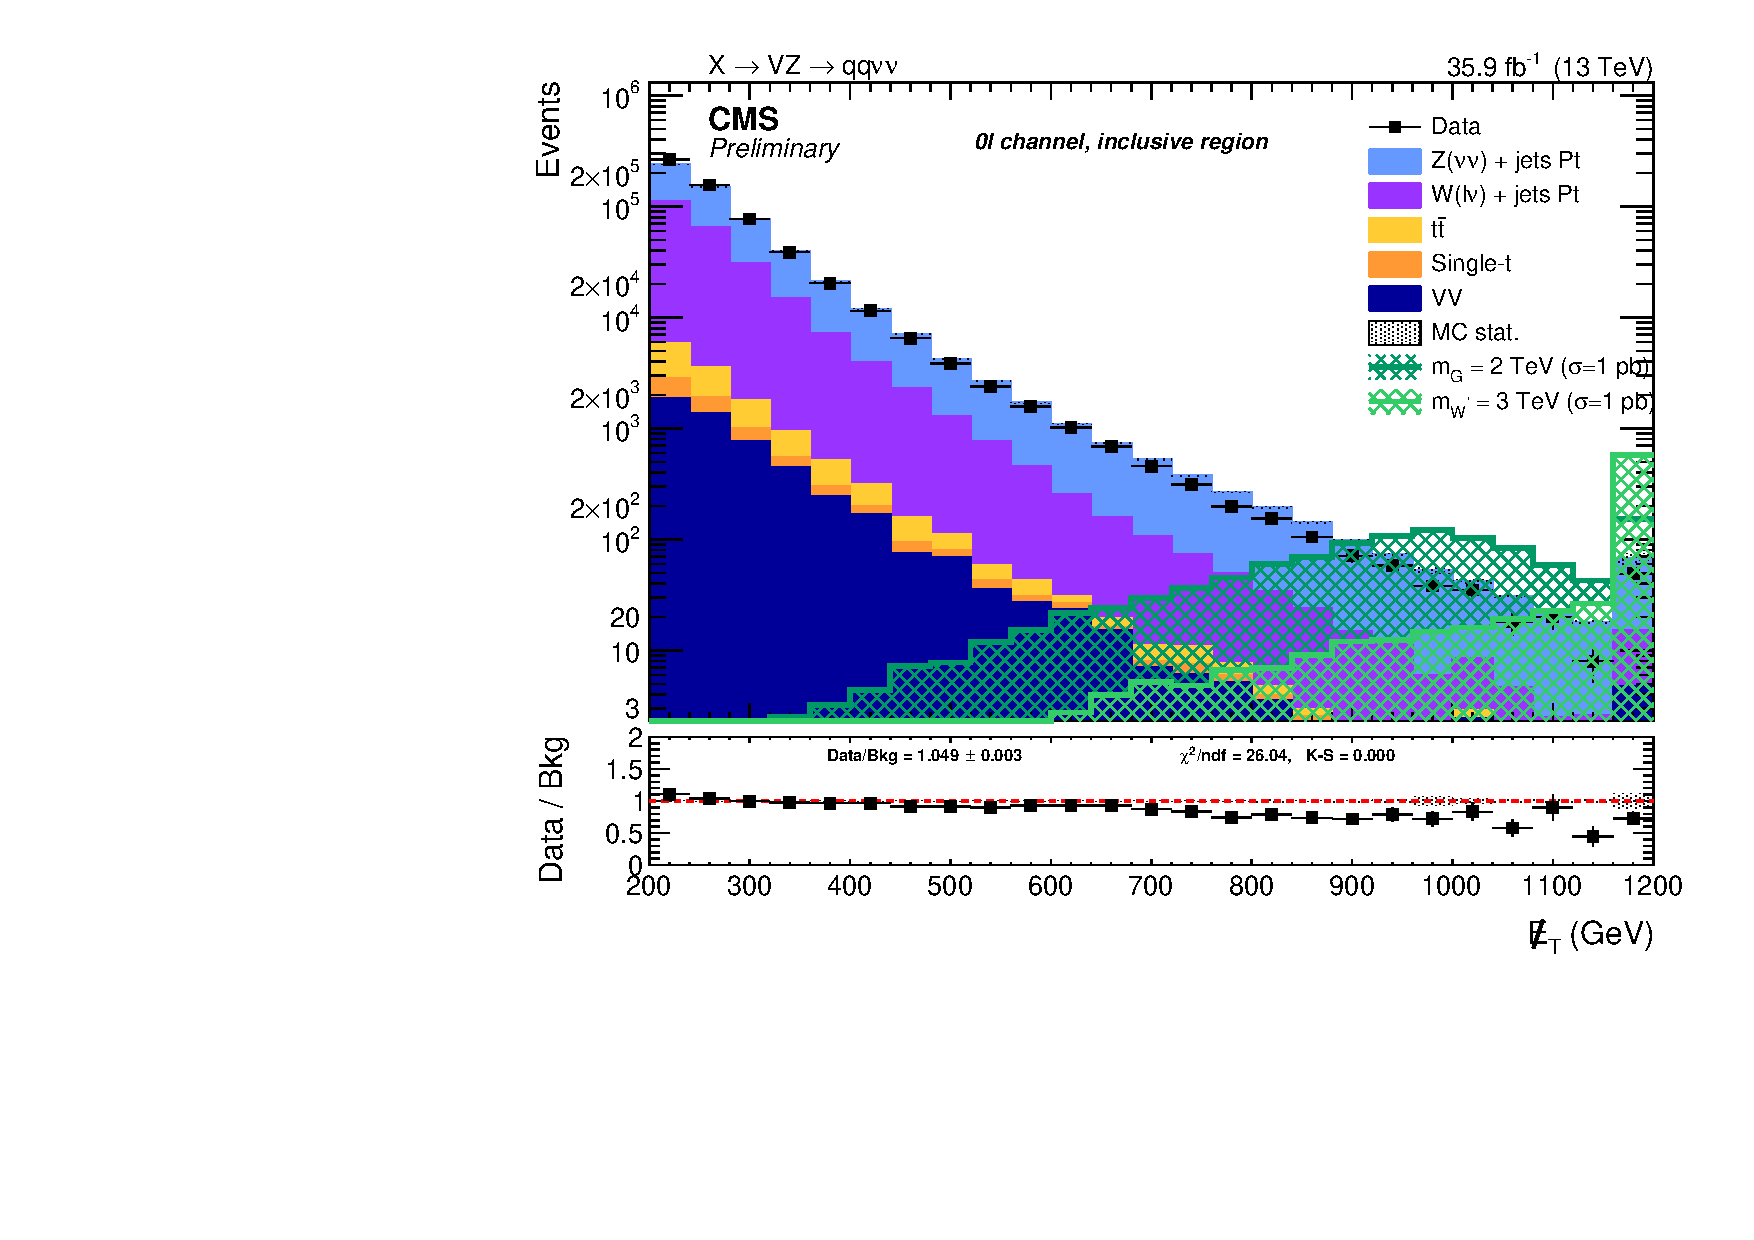
\includegraphics[width=.495\textwidth]{plots/v9_U/XVZnnInc/MEt_pt.pdf}
     %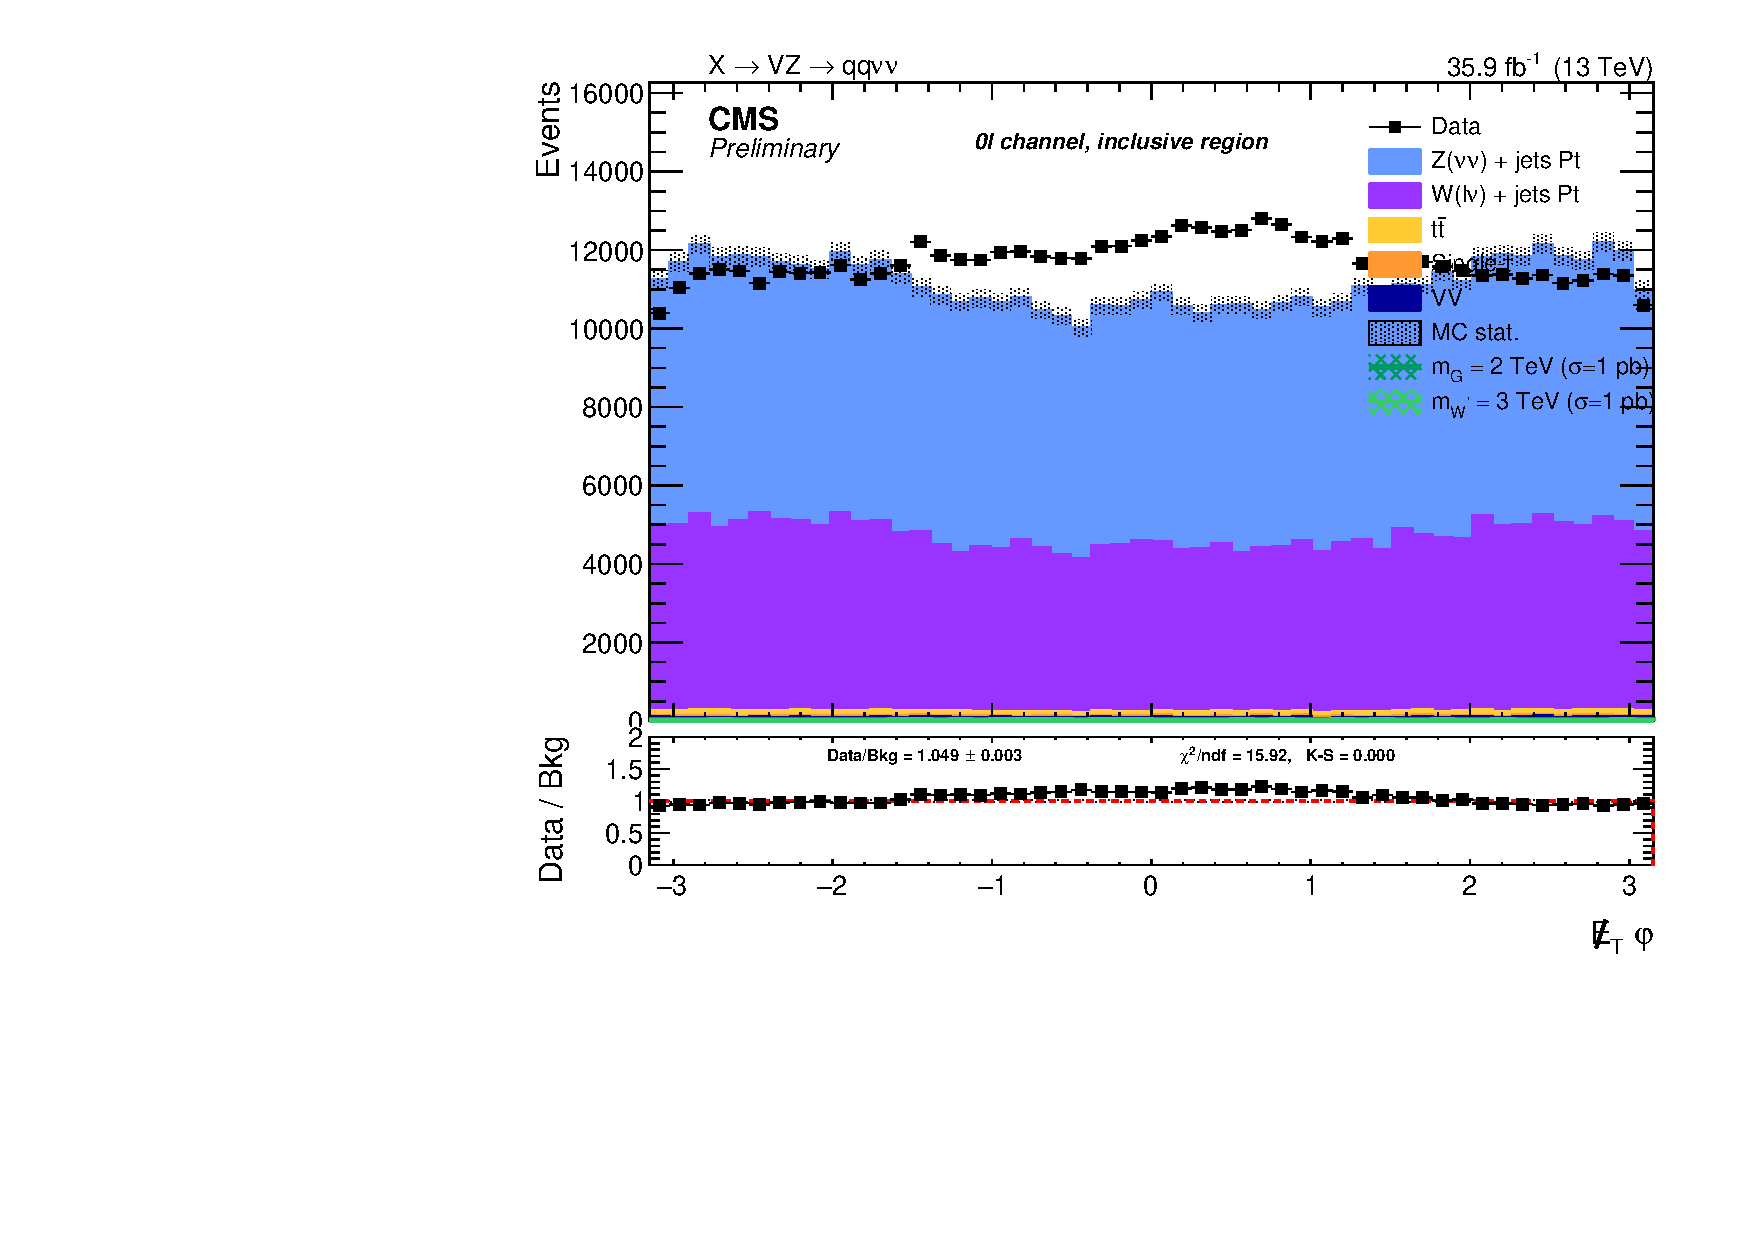
\includegraphics[width=.495\textwidth]{plots/v9_U/XVZnnInc/MEt_phi.pdf}
   
   \caption{Type-1 corrected \MET distribution after inclusive selections.}
   \label{fig:type1_met}
 \end{figure}


\clearpage

